% Time-stamp: <2022-11-10 13:50:02 A13258Q>
% Romain Lafarguette 2020, https://romainlafarguette.github.io/

%% ---------------------------------------------------------------------------
%% Preamble: Packages and Setup
%% ---------------------------------------------------------------------------
% Class 
\documentclass{beamer}

% Theme
\usetheme{Boadilla}
\usecolortheme{dolphin}
%\setbeamertemplate{headline}{} % Remove the top navigation bar

% Font and encoding
\usepackage[utf8]{inputenc} % Input font
\usepackage[T1]{fontenc} % Output font
\usepackage{lmodern} % Standard LateX font
\usefonttheme{serif} % Standard LateX font

% Maths 
\usepackage{amsfonts, amsmath, mathabx, bm, bbm} % Maths Fonts

% Graphics
\usepackage{graphicx} % Insert graphics
\usepackage{subfig} % Multiple figures in one graphic
\graphicspath{{/../static/img}{/../static/diagrams}}

% Layout
\usepackage{changepage}

% Colors
\usepackage{xcolor}
\definecolor{imfblue}{RGB}{0,76,151} % Official IMF color
\setbeamercolor{title}{fg=imfblue}
\setbeamercolor{frametitle}{fg=imfblue}
\setbeamercolor{structure}{fg=imfblue}

% Tables
\usepackage{booktabs,rotating,multirow} % Tabular rules and other macros
%\usepackage{pdflscape,afterpage} % Landscape mode and afterpage
%\usepackage{threeparttable} % Split long tables
\usepackage[font=scriptsize,labelfont=scriptsize,labelfont={color=imfblue}]{caption}

% Import files
\usepackage{import}

% Appendix slides
\usepackage{appendixnumberbeamer} % Manage page numbers for appendix slides

% References
\usepackage{hyperref}

% A few macros: environments
\newenvironment{wideitemize}{\itemize\addtolength{\itemsep}{10pt}}{\enditemize}
\newenvironment{wideenumerate}{\enumerate\addtolength{\itemsep}{10pt}}{\endenumerate}

\newenvironment{extrawideitemize}{\itemize\addtolength{\itemsep}{30pt}}{\enditemize}
\newenvironment{extrawideenumerate}{\enumerate\addtolength{\itemsep}{30pt}}{\endenumerate}

% Remove navigation symbols and other superfluous elements
\setbeamertemplate{navigation symbols}{}
\beamertemplatenavigationsymbolsempty

%\setbeamertemplate{note page}[plain]
\hypersetup{pdfpagemode=UseNone} % don't show bookmarks on initial view
\setbeameroption{hide notes}

% Institute font
\setbeamerfont{institute}{size=\footnotesize}
\DeclareMathSizes{10}{9}{7}{5}  

%% ---------------------------------------------------------------------------
%% Title info
%% ---------------------------------------------------------------------------
\title[Advanced Models]{Advanced Forecasting Models}
\author[R. Lafarguette]{Romain Lafarguette, Ph.D. }
\institute[IMF STX]{Quant \& IMF External Expert\thanks{\scriptsize{\emph{This training material is the property of the International Monetary Fund (IMF) and is intended for use in IMF courses. Any reuse requires the permission of the IMF.}}} \\
\begin{center}{\href{https://romainlafarguette.github.io/}{\textcolor{imfblue}{https://romainlafarguette.github.io/}}} \end{center}} 

\date[STI, 10 Nov 2022]{Singapore Training Institute, 10 November 2022}

\titlegraphic{\vspace{-0.75cm}
    \begin{figure}
    \centering
    \subfloat{{
\includegraphics[width=2cm]{../static/img/imf_logo}}}%
    \end{figure}}


% Slide between sections
\AtBeginSection[]
{
    \begin{frame}
        \frametitle{Table of Contents}
        \tableofcontents[currentsection]
    \end{frame}
}

%% ---------------------------------------------------------------------------
%% Title slide
%% ---------------------------------------------------------------------------
\begin{document}

\begin{frame}
\maketitle
\end{frame}


%% ---------------------------------------------------------------------------
%% TO IMPROVE: The entire EWMA section, the code of a slide in GARCH copy-pasted from Hurlin
%% TODO: Add other GARCH models (EGARCH, etc.), Add GARCH with exogeneous regressors
%% TODO: Add the GARCH picture from the liquidity forecasting framework too
%% TODO: Add Nemenyi test
%% ---------------------------------------------------------------------------
\section{Advanced Seasonal Models}

\begin{frame}
 \frametitle{Bias Identification}
  \makebox[\linewidth]{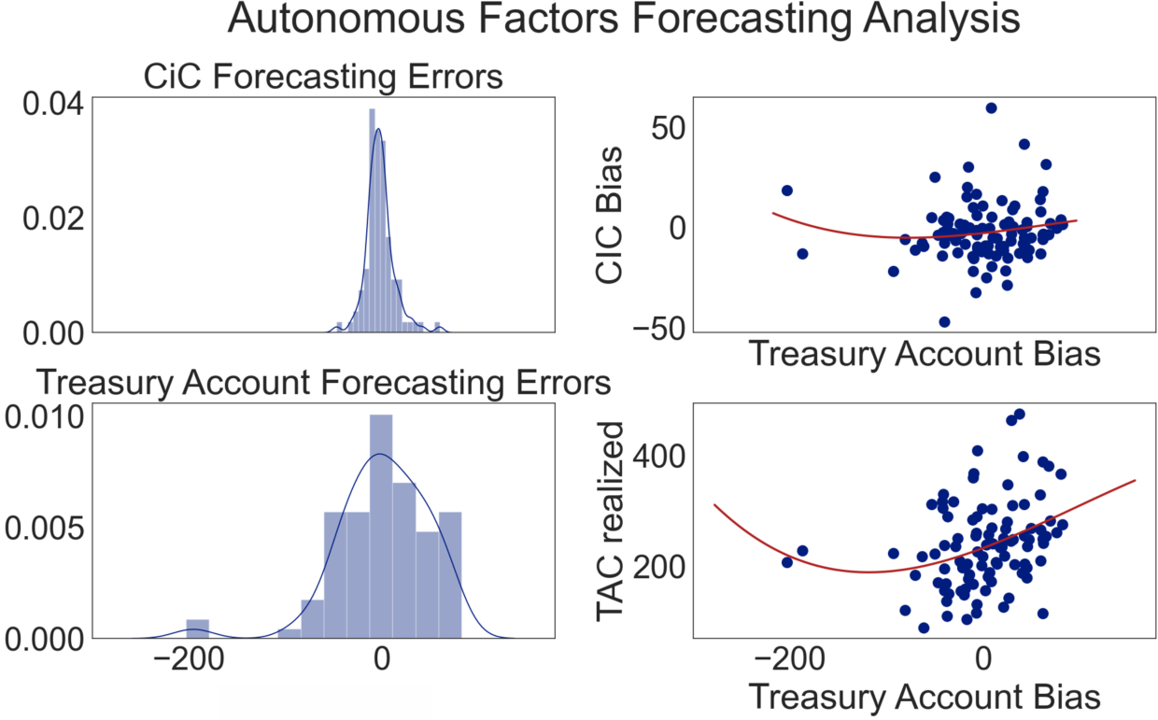
\includegraphics[width=0.85\paperwidth]{../static/course_3_img/bias_correction.png}}
 \hspace*{15pt}\hbox{\scriptsize Credit:\thinspace{\scriptsize\itshape Author}}      
 \end{frame}


  \begin{frame}
    \frametitle{Advanced Models Typology}

  \begin{wideitemize}
    \item \textbf{ETS with trigonometric} multiple seasonalities and indicators for events
    \item \textbf{ARIMA with trigonometric} multiple seasonalities and indicators for events
    \item \textbf{ARIMA with stochastic} multiple seasonalities and indicators for events
    \item \textbf{TBATS} – a state space model with exponential smoothing, stochastic trigonometric patterns, Cox-Box transformation and ARIMA errors. TBATS cannot incorporate events 
    \item \textbf{Composite TBATS} – where the local level and events are modelled with ETS and the seasonality/trend with TBATS
    \end{wideitemize}
    
  \end{frame}
  

    \begin{frame}
      \frametitle{Box Cox Transformation}

      \begin{wideitemize}
        \item The Box-Cox transformation is used to transform non-Gaussian data $y_t$ into Gaussian  data
        \item Working with Gaussian data makes it easier to apply the standard model in econometrics
        \item The Box Cox transformation works with a parameters $\lambda$ that takes values between $[-5, 5]$

        \item For positive $y_t$ data:
          \begin{itemize}
          \item $y(\lambda) = \frac{y^{\lambda}-1}{\lambda}$ if $\lambda neq 0$
          \item $\text{log}(y)$ if $\lambda = 0$
          \end{itemize}

        \item For negative $y_t$ data, use an extra parameter $\lambda_2$ 
          \begin{itemize}
          \item $y(\lambda) = \frac{(y + \lambda_2)^{\lambda}-1}{\lambda}$ if $\lambda neq 0$
          \item $\text{log}(y + \lambda_2)$ if $\lambda = 0$
          \end{itemize}          
      \end{wideitemize}      
    \end{frame}


    \begin{frame}
      \frametitle{Transforming Data with the Box Cox Transformation}
  \makebox[\linewidth]{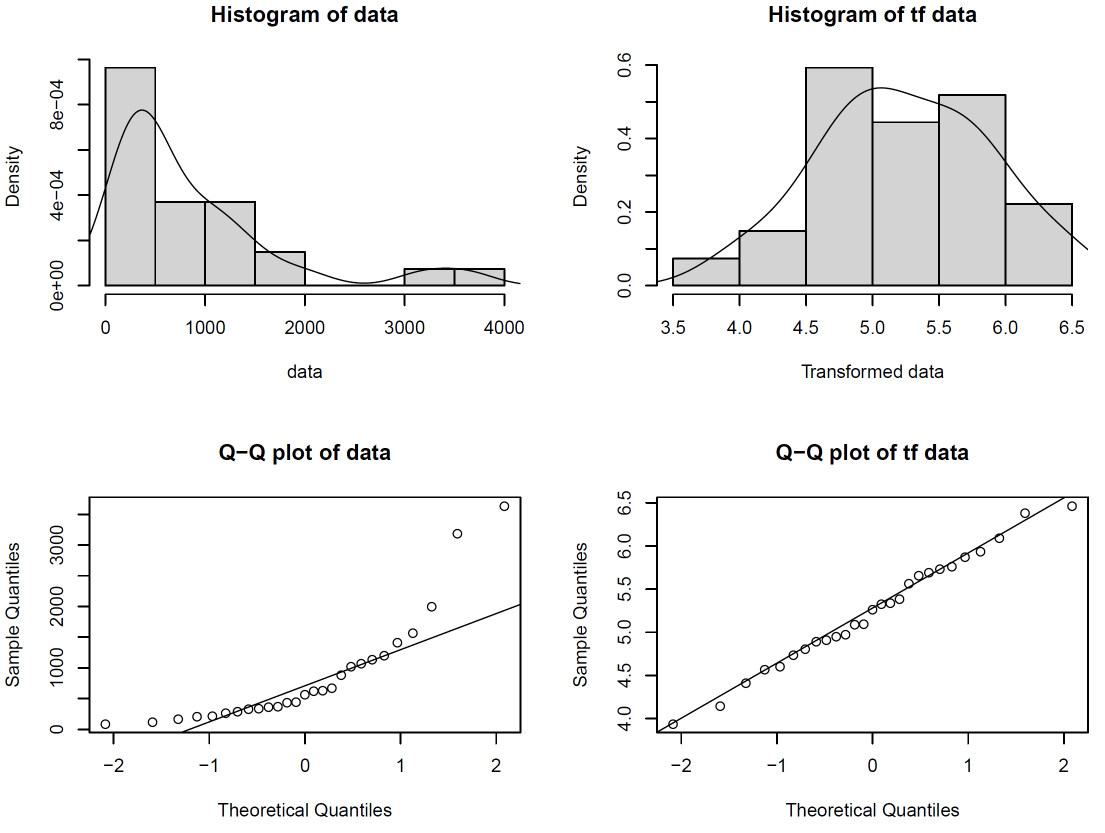
\includegraphics[width=0.75\paperwidth]{../static/course_3_img/box_cox_data_transformation.PNG}}
  \hspace*{15pt}\hbox{\scriptsize Credit:\thinspace{\scriptsize\itshape https://universeofdatascience.com/}}      
    \end{frame}

    \begin{frame}
      \frametitle{The TBATS Model: Overview}
  \makebox[\linewidth]{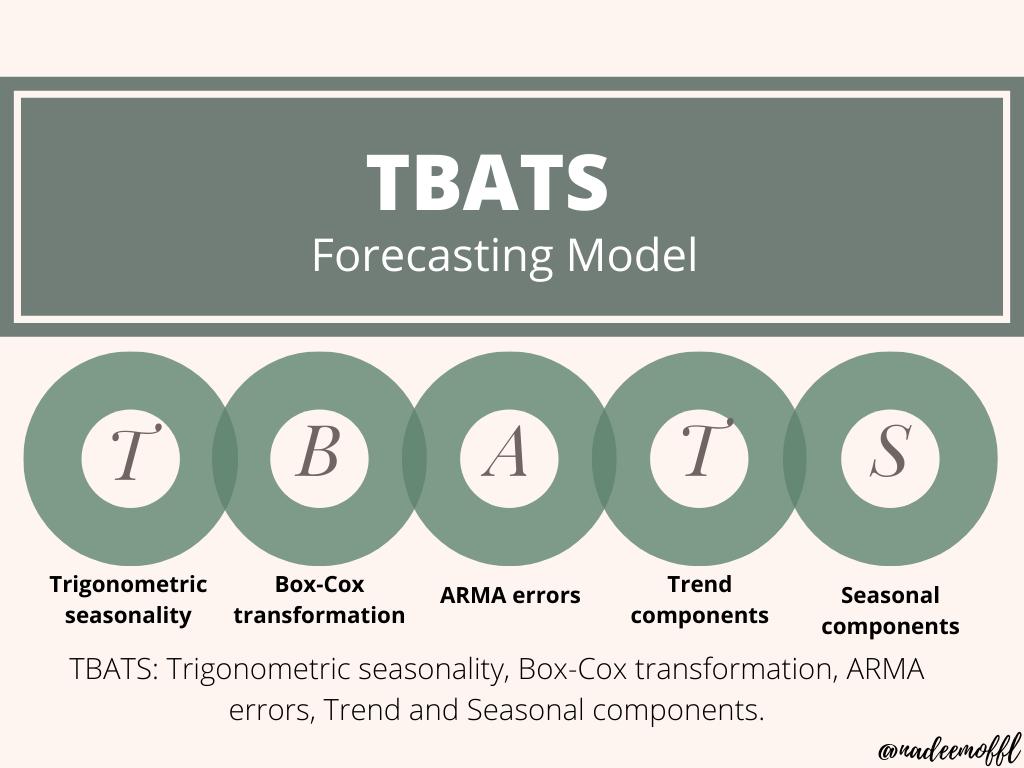
\includegraphics[width=0.75\paperwidth]{../static/course_3_img/TBATS presentation.png}}
  \hspace*{15pt}\hbox{\scriptsize Credit:\thinspace{\scriptsize\itshape https://medium.com/analytics-vidhya/}}      
    \end{frame}

    
  \begin{frame}
    \frametitle{The TBATS Model: Overview}

    \begin{wideitemize}
    \item Combines in a \textbf{single state-space} model:

      \begin{itemize}
      \item Trigonometric terms to account for seasonality
      \item Box-Cox transformation to account for non-normality and heterogeneity
      \item ARIMA errors to model the residuals short-term dynamic
      \item Trend (potentially damped)        
      \item Seasonal (including multiple and non-integer period)
      \end{itemize}

    \item Main specifications:
      \begin{itemize}
      \item Handles non-integer seasonality, multiple seasonal periods
      \item Entirely automated
      \item Predictions interval often wide
      \item Very slow on long series
      \end{itemize}      
    \end{wideitemize}
    \end{frame}

    
    \begin{frame}
      \frametitle{The TBATS Model: Specification}
  \makebox[\linewidth]{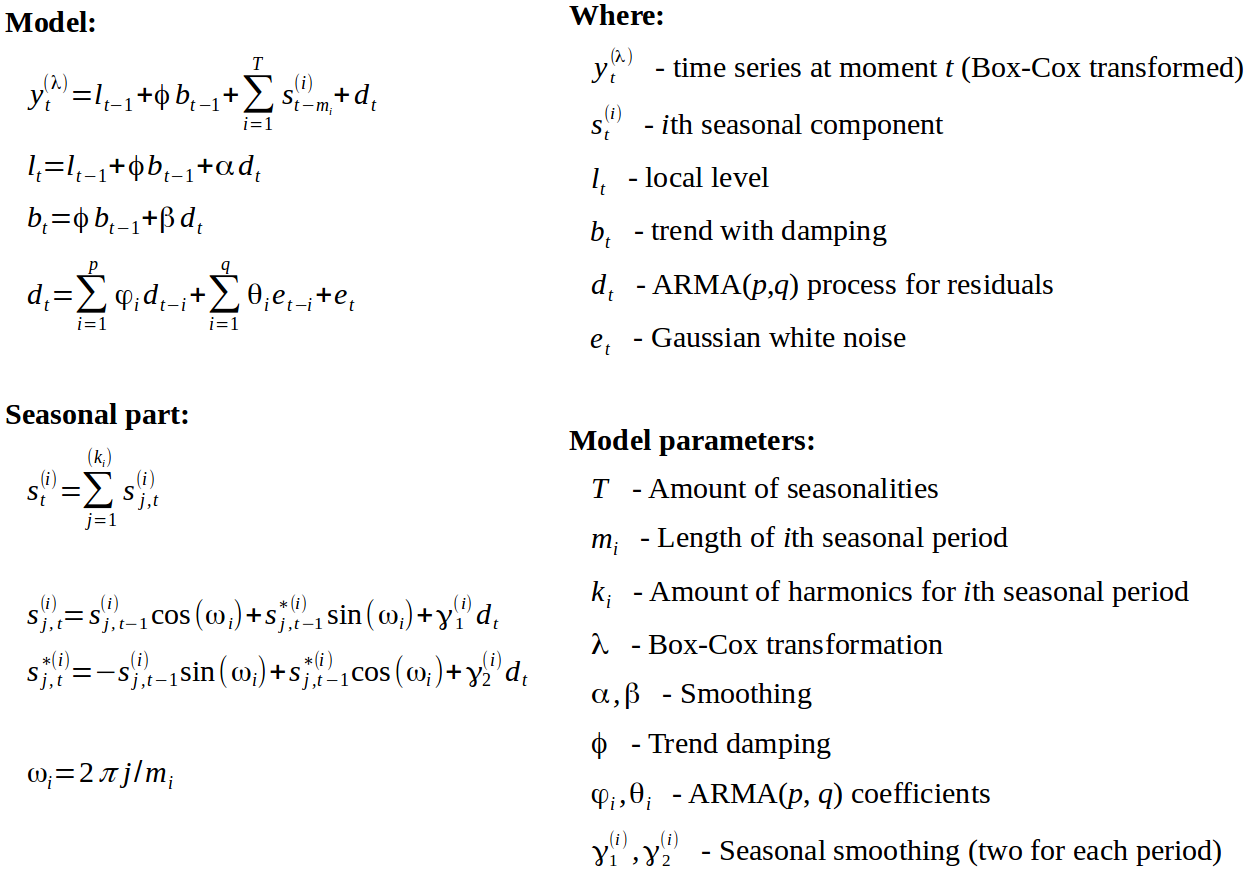
\includegraphics[width=0.75\paperwidth]{../static/course_3_img/TBATS_specification.png}}
  %\hspace*{15pt}\hbox{\scriptsize Credit:\thinspace{\scriptsize\itshape Author}}      
    \end{frame}

    \begin{frame}
      \frametitle{The TBATS Model: Decomposition}
  \makebox[\linewidth]{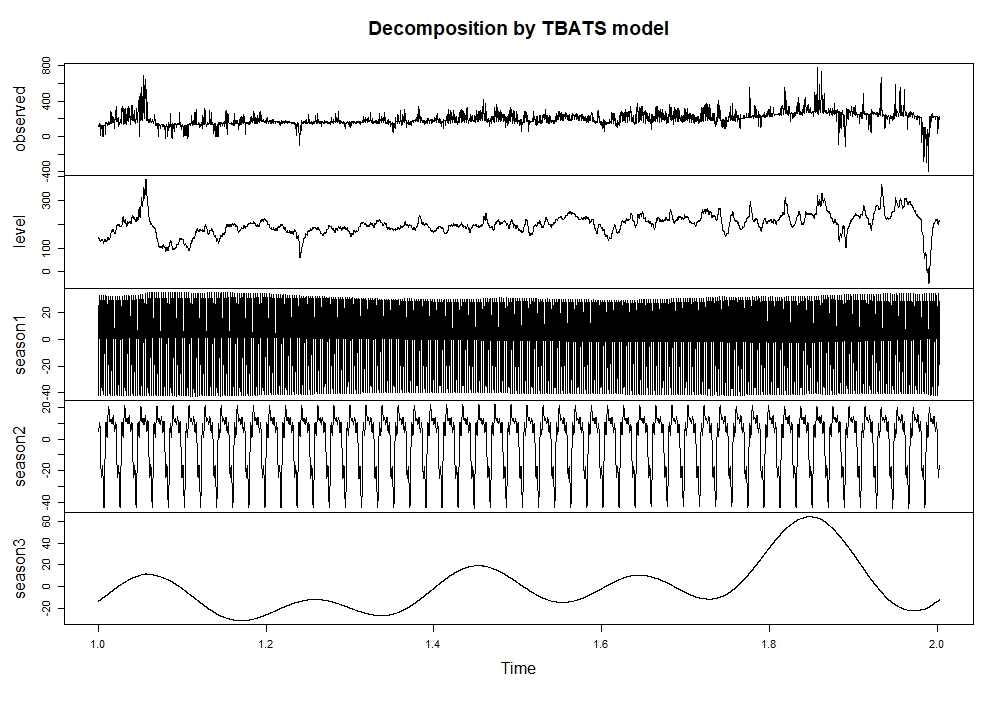
\includegraphics[width=0.75\paperwidth]{../static/course_3_img/TBATS_decomposition.jpg}}
  %\hspace*{15pt}\hbox{\scriptsize Credit:\thinspace{\scriptsize\itshape Author}}      
    \end{frame}


\section{Volatility Models: EWMA and GARCH Models}

\begin{frame}
  \frametitle{Volatility Estimation}
  \makebox[\linewidth]{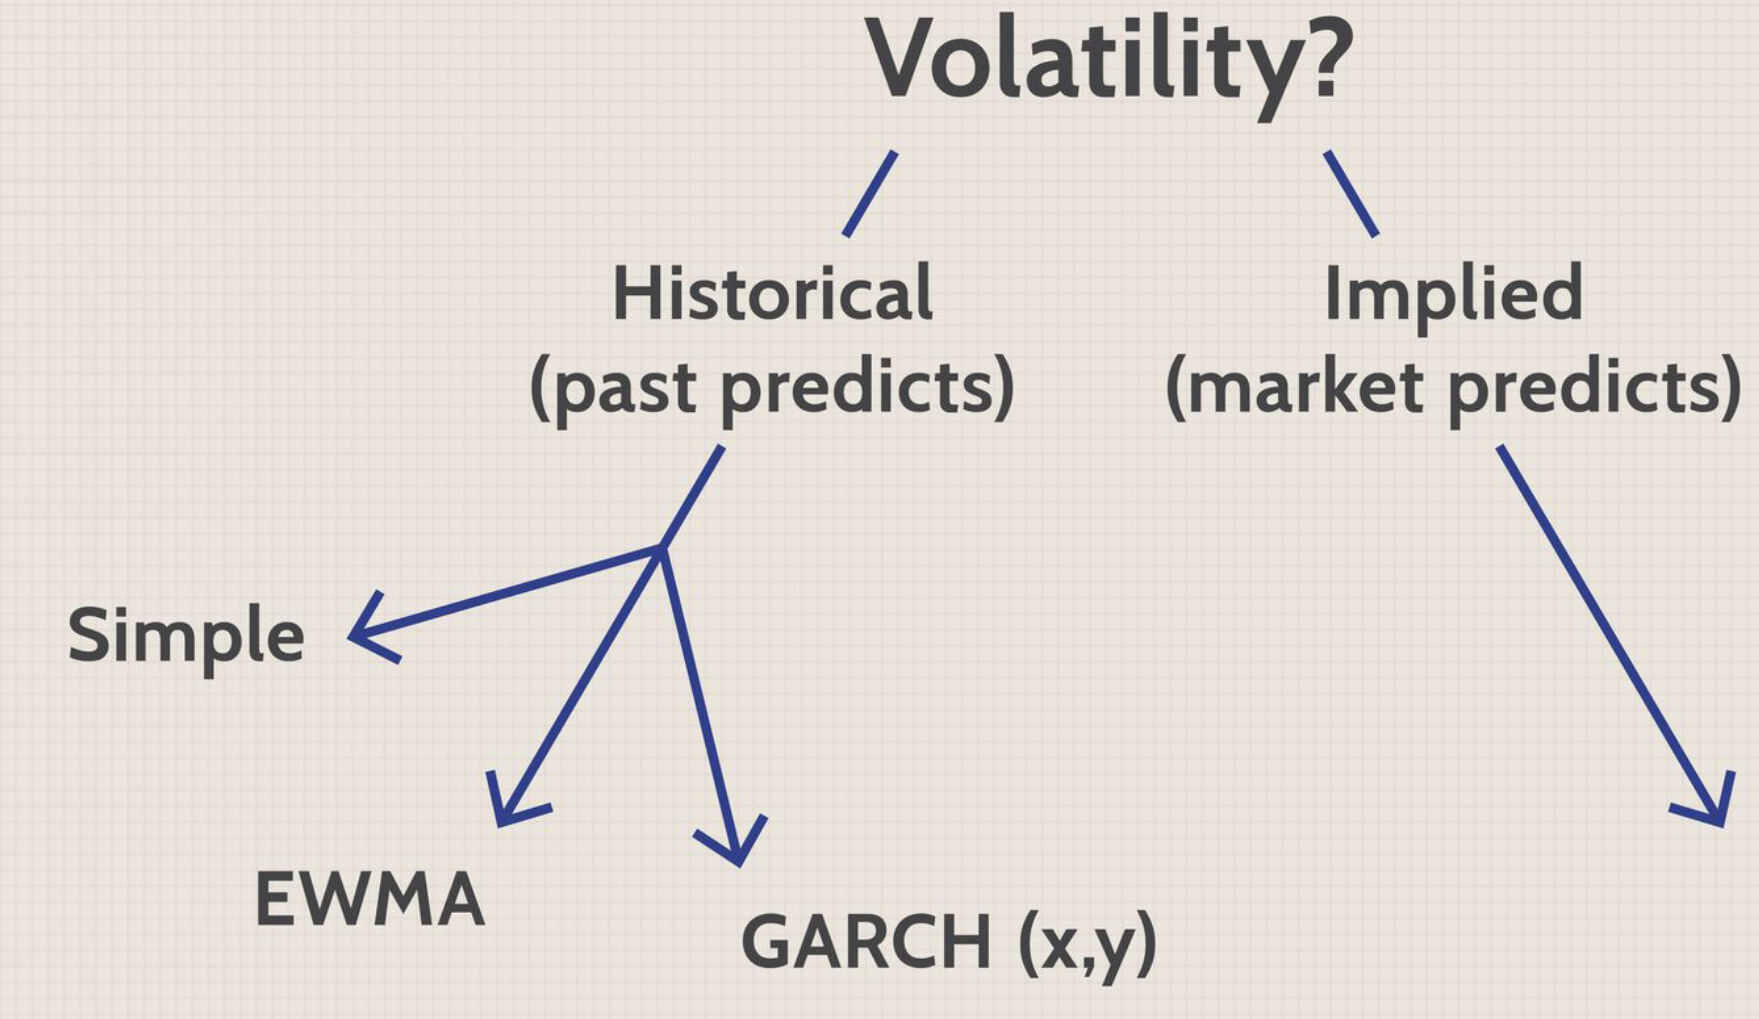
\includegraphics[width=0.75\paperwidth]{../static/course_3_img/volatility_decision_tree.PNG}}
  \hspace*{15pt}\hbox{\scriptsize Credit:\thinspace{\scriptsize\itshape Sabrina Jiang}}          
  
\end{frame}

\begin{frame}
  \frametitle{EWMA Model}
  \makebox[\linewidth]{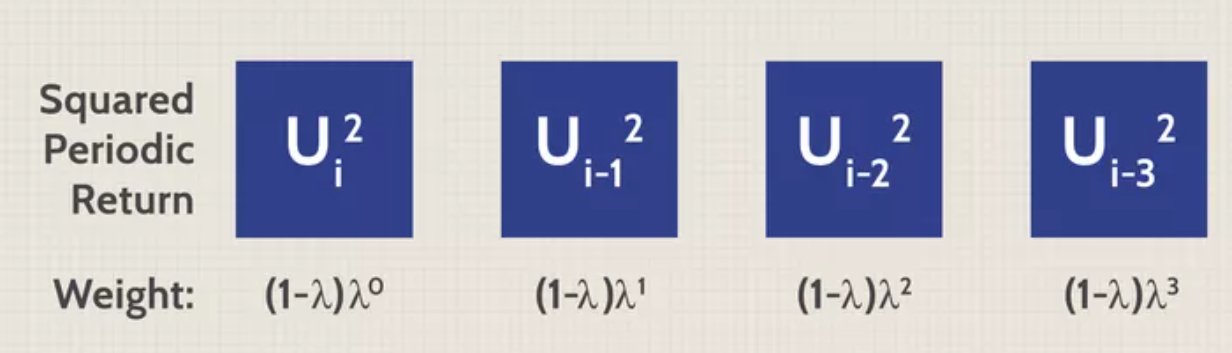
\includegraphics[height=0.35\paperheight]{../static/course_3_img/ewma_squared_returns.PNG}}
  \hspace*{15pt}\hbox{\scriptsize Credit:\thinspace{\scriptsize\itshape Sabrina Jiang}}          

  \medskip

  \makebox[\linewidth]{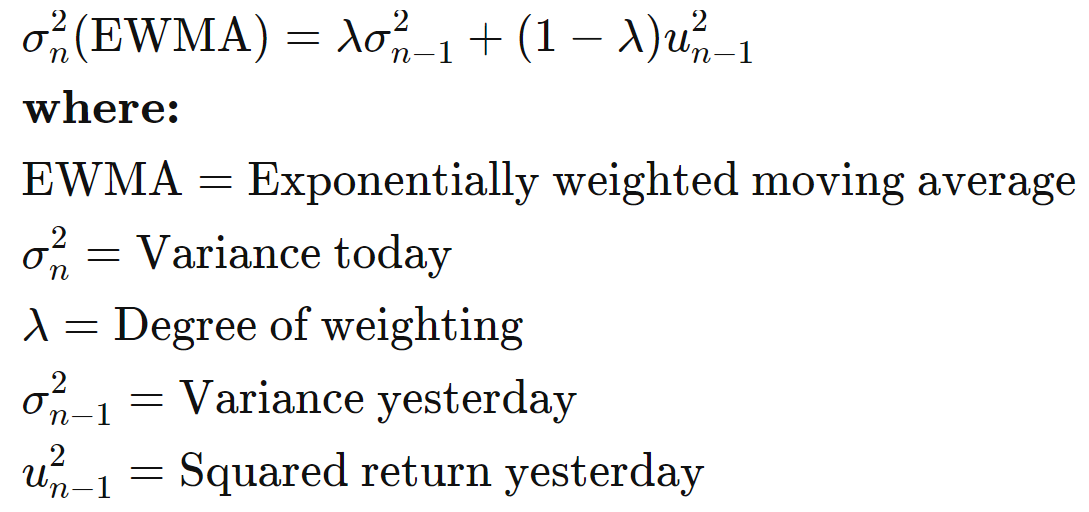
\includegraphics[height=0.35\paperheight]{../static/course_3_img/ewma_formula.PNG}}
  %\hspace*{15pt}\hbox{\scriptsize Credit:\thinspace{\scriptsize\itshape Sabrina Jiang}}          
  
\end{frame}


\begin{frame}
  \frametitle{EWMA Weights}
  \makebox[\linewidth]{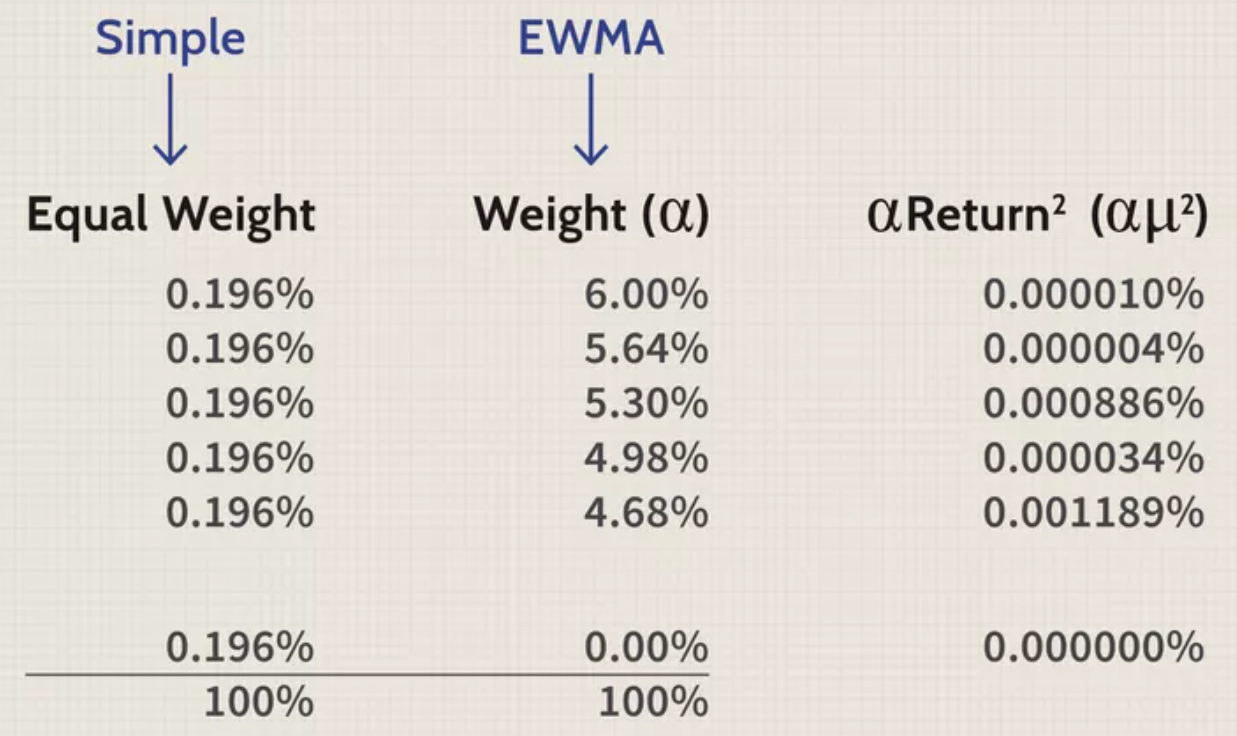
\includegraphics[height=0.65\paperheight]{../static/course_3_img/ewma_weights.PNG}}
  %\hspace*{15pt}\hbox{\scriptsize Credit:\thinspace{\scriptsize\itshape Sabrina Jiang}}            
\end{frame}


\begin{frame}
  \frametitle{Homoscedasticity and Heteroscedasticity}
  \makebox[\linewidth]{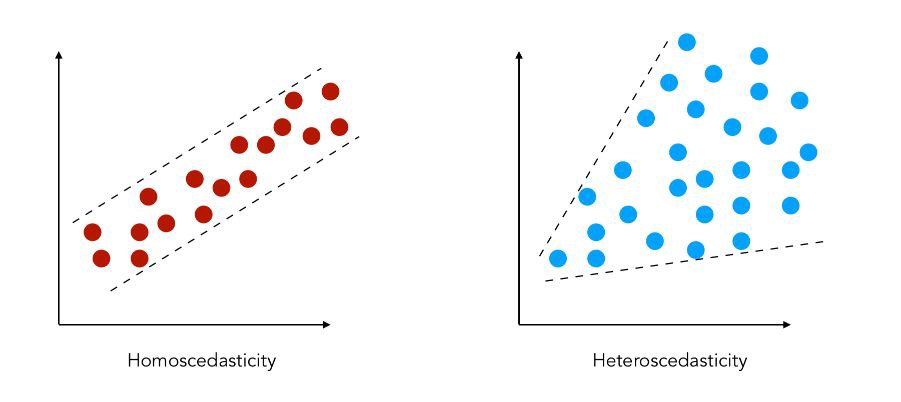
\includegraphics[width=0.95\paperwidth]{../static/course_3_img/homo_hsk.jpeg}}
  \hspace*{15pt}\hbox{\scriptsize Credit:\thinspace{\scriptsize\itshape Medium.com}}          
\end{frame}

\begin{frame}
  \frametitle{GARCH Models}

  \begin{alertblock}{Meaning}
    \textbf{GARCH}: \textbf{G}eneralized \textbf{A}uto\textbf{R}egressive \textbf{C}onditional \textbf{H}eteroscedasticity    \    
  \end{alertblock}

\medskip
  
\emph{Reference: Bollerslev, T. (1986), Generalized Autoregressive Conditional Heteroskedasticity. Journal of
  Econometrics, 31, 307-327}\\

\end{frame}


\begin{frame}
\begin{block}{Definition: GARCH Model}

  The stochastic process $\{ \epsilon_t, \ t \ in \mathbb{Z} \}$ is said to be a \textbf{GARCH}(p,q) process if:

  \begin{equation*}
    \epsilon_t = Z_t \sigma_t
  \end{equation*}

  \medskip

  where $Z_t$ is a sequence of i.i.d variables with $\mathbb{E}(Z_t) = 0$ and $\mathbb{V}(Z_t) = 1$, and $\sigma_t$ is a non-negative process such that:
  \begin{equation*}
    \sigma^2_t = \omega + \sum^p_{i=1} \alpha_i \epsilon^2_{t-i} + \sum^p_{i=1} \beta_i \sigma^2_{t-i}
  \end{equation*}

  \medskip

  with $\omega >0$, $\forall \ i, (\alpha_i, \beta_i) \ \in \ \mathbb{R}^{+,2}$ and $\sum^p_{i=1} \alpha_i + \sum^p_{i=1} \beta_i <1$  
\end{block}
\end{frame}


\begin{frame}
  \frametitle{GARCH: Intuition}
  \begin{wideitemize}
  \item The conditional variance of a GARCH(p, q) depends on:
    \begin{itemize}
    \item The first p lag of the $\epsilon_t^2$ (e.g. the squared error terms)
    \item The first $q$ lag of the conditional variance $\sigma^2$
    \end{itemize}

 \begin{equation*}
    \sigma^2_t = \omega + \underbrace{\sum^p_{i=1} \alpha_i \epsilon^2_{t-i}}_{\text{ARCH Components}} + \underbrace{\sum^p_{i=1} \beta_i \sigma^2_{t-i}}_{GARCH components}
  \end{equation*}
    
   
  \item The parameters $\alpha_i$ are often called the \textbf{ARCH parameters}
  \item The parameters $\beta_i$ are often called the \textbf{GARCH parameters}
\end{wideitemize}
  
\end{frame}

\begin{frame}
  \frametitle{GARCH(1, 1)}

  \begin{alertblock}{Tip}
GARCH(1,1) specifications are generally sufficient to capture the dynamics of the conditional variance
  \end{alertblock}

  \medskip
  
\begin{block}{Special Case: GARCH(1, 1)}

  The stochastic process $\{ \epsilon_t, \ t \ in \mathbb{Z} \}$ is said to be a \textbf{GARCH}(1,2) process if:

  \begin{equation*}
    \epsilon_t = Z_t \sigma_t
  \end{equation*}

  \medskip

  where $Z_t$ is a sequence of i.i.d variables with $\mathbb{E}(Z_t) = 0$ and $\mathbb{V}(Z_t) = 1$, and $\sigma_t$ is a non-negative process such that:
  \begin{equation*}
    \sigma^2_t = \omega + \alpha \epsilon^2_{t-1} + \beta \sigma^2_{t-1}
  \end{equation*}

  \medskip

  with $\omega >0$, $\alpha \geq 0, \beta \geq 0$ and $\alpha + \beta <1$  
\end{block}
\end{frame}


\begin{frame}
  \frametitle{Conditional Variance Persistences: Intrinsic and Extrinsic}
  \begin{itemize}
  \item The conditional variance $\sigma_t^2 = \omega + \alpha \epsilon^2_{t-1} + \beta \sigma^2_{t-1}$ depends on two effects:
    \begin{itemize}
    \item An \textbf{intrinsic persistence} effect through the first lag of the conditional variance
    \item An \textbf{extrinsic persistence} effect
    \end{itemize}
    
  \item Following a positive (or negative) shock at time \emph{t-1}, the conditional variance at time \emph{t} increases (impact effect) and thus it has an impact on $\epsilon_t = Z_t \sigma_t$

    \begin{equation*}
      \text{shock} \ z_{t-1} \ > \ 0 \Rightarrow \ \epsilon_{t-1} \ \uparrow \ \Rightarrow \ \sigma_t \ \uparrow \ \dots
    \end{equation*}

  \item Starting from the next period (at time $t$), the effect of the shock at $t-1$ on the conditional variance at $t+1$ passes through the conditional variance at time $t$ (intrisic persistence)

    \begin{equation*}
      \text{shock} \ z_{t-1} \ \Rightarrow \ \sigma_t \ \uparrow \ \Rightarrow \ \sigma^2_{t+1} \ \uparrow 
    \end{equation*}
\item The overall effect of a shock can be decomposed into a \textbf{contemporaneous effect}, which depends on $\alpha$ and a \textbf{persistence effect} that depends on $\beta$
    
  \end{itemize}
\end{frame}



\begin{frame}
  \frametitle{Remarks}

  \begin{wideitemize}
  \item It is often the case that:
      \begin{wideenumerate}
  \item The sum of the estimates of $\alpha$ and $\beta$ are generally close (but below 1)
  \item The estimate of $\beta$ is generally greater than the one of $\alpha$
  \item The estimate of $\beta$ is generally larger than 0.90 for daily returns and the estimate of $\alpha$ is below 0.1
  \end{wideenumerate}
  \item Be careful: it is not a general rule, just an observation.
  \end{wideitemize}  
\end{frame}

\begin{frame}
  \frametitle{GARCH Extensions}
  \begin{wideitemize}
  \item I won't cover them during the course but many extensions have been proposed to extend the GARCH model, including model for dealing with \textbf{asymmetric responses}, \textbf{persistence} and \textbf{long-memory}
    \begin{wideitemize}
      \item \textbf{IGARCH model}: Integrated GARCH (model persistence)
      \item \textbf{GARCH-M model}: GARCH mean, when the mean depends on the volatility
      \item \textbf{GJR-GARCH model}: Glosten, Jagannathan and Runkle (1993): asymmetric with non-linearities
      \item \textbf{TGARCH model}: Threshold GARCH captures regimes change
      \item \textbf{EGARCH model}: Exponential GARCH captures asymmetric responses and big shocks
    \end{wideitemize}
  \end{wideitemize}
\end{frame}


\begin{frame}
  \frametitle{Application: FX Modeling}
  \makebox[\linewidth]{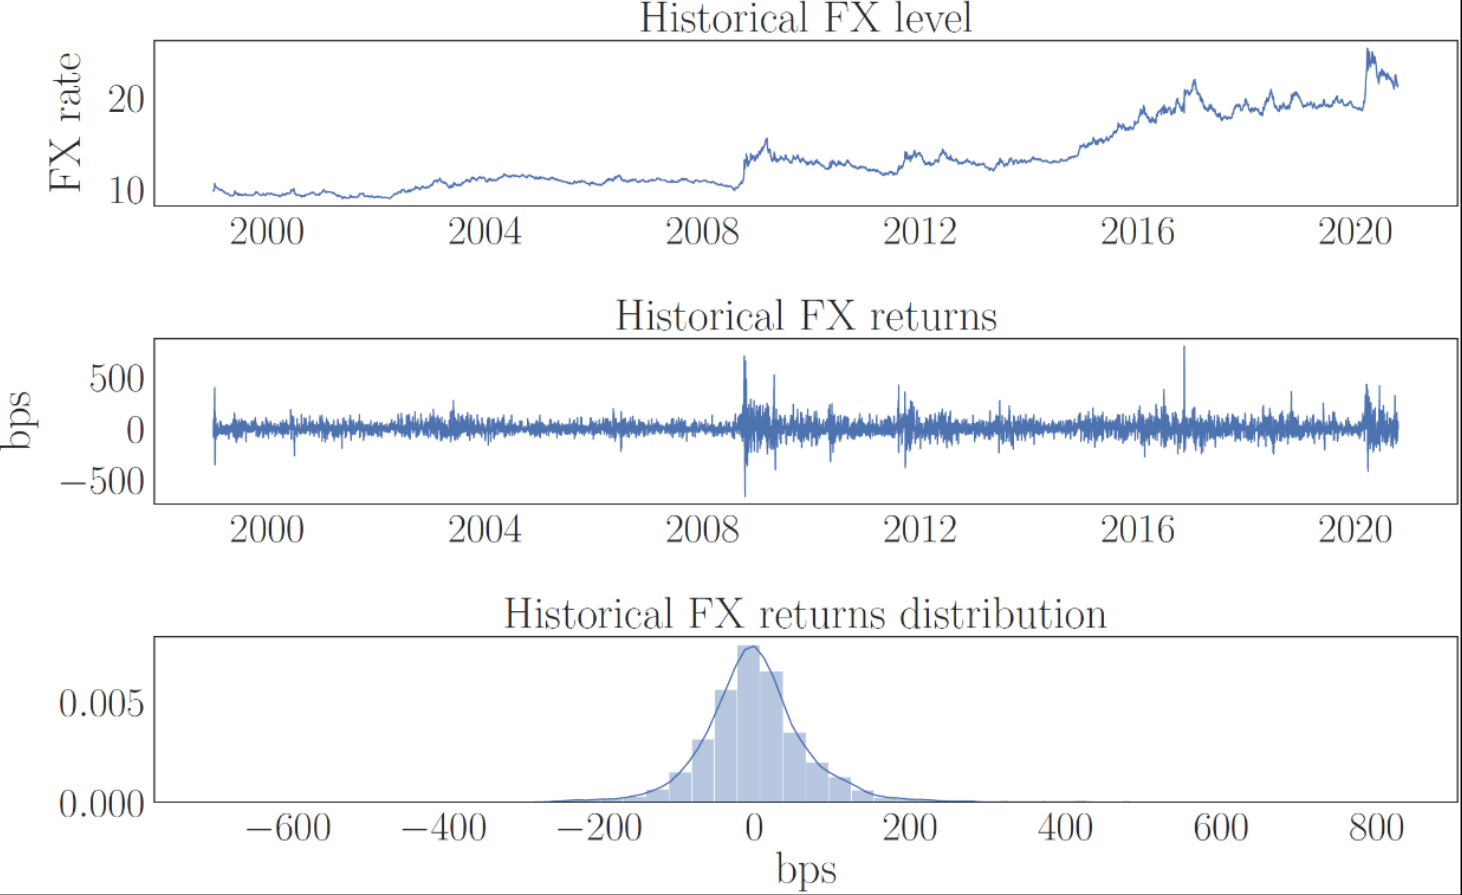
\includegraphics[width=0.85\paperwidth]{../static/course_3_img/var_fxi_stat_desc.PNG}}
  \hspace*{15pt}\hbox{\scriptsize Credit:\thinspace{\scriptsize\itshape Lafarguette and Veyrune (2021)}}          
\end{frame}


\begin{frame}
  \frametitle{Application: GARCH Estimation}
  \makebox[\linewidth]{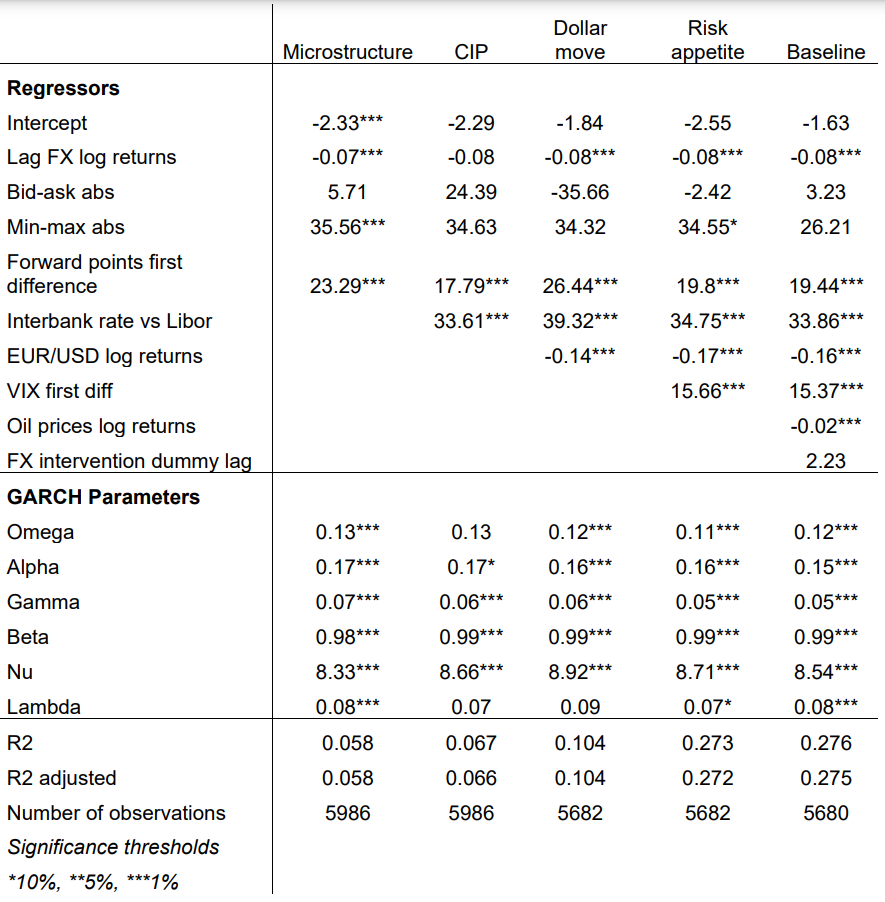
\includegraphics[width=0.6\paperwidth]{../static/course_3_img/GARCH_estimation_table.PNG}}
  \hspace*{15pt}\hbox{\scriptsize Credit:\thinspace{\scriptsize\itshape Lafarguette and Veyrune (2021)}}          
\end{frame}

\begin{frame}
  \frametitle{Application: MXN/USD Conditional Volatility}
  \makebox[\linewidth]{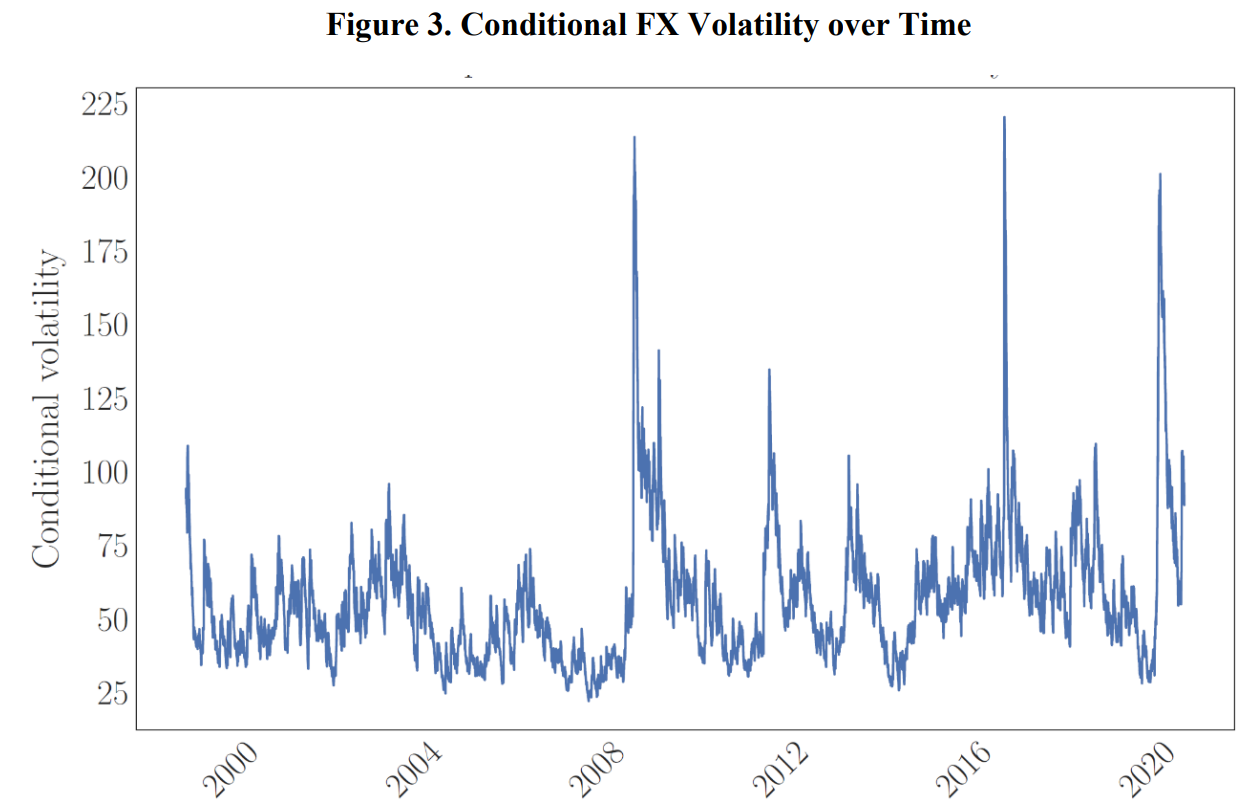
\includegraphics[width=0.85\paperwidth]{../static/course_3_img/var_fxi_conditional_vol.PNG}}
  \hspace*{15pt}\hbox{\scriptsize Credit:\thinspace{\scriptsize\itshape Lafarguette and Veyrune (2021)}}          
\end{frame}

\begin{frame}
  \frametitle{Application: MXN/USD Conditional Density}
  \makebox[\linewidth]{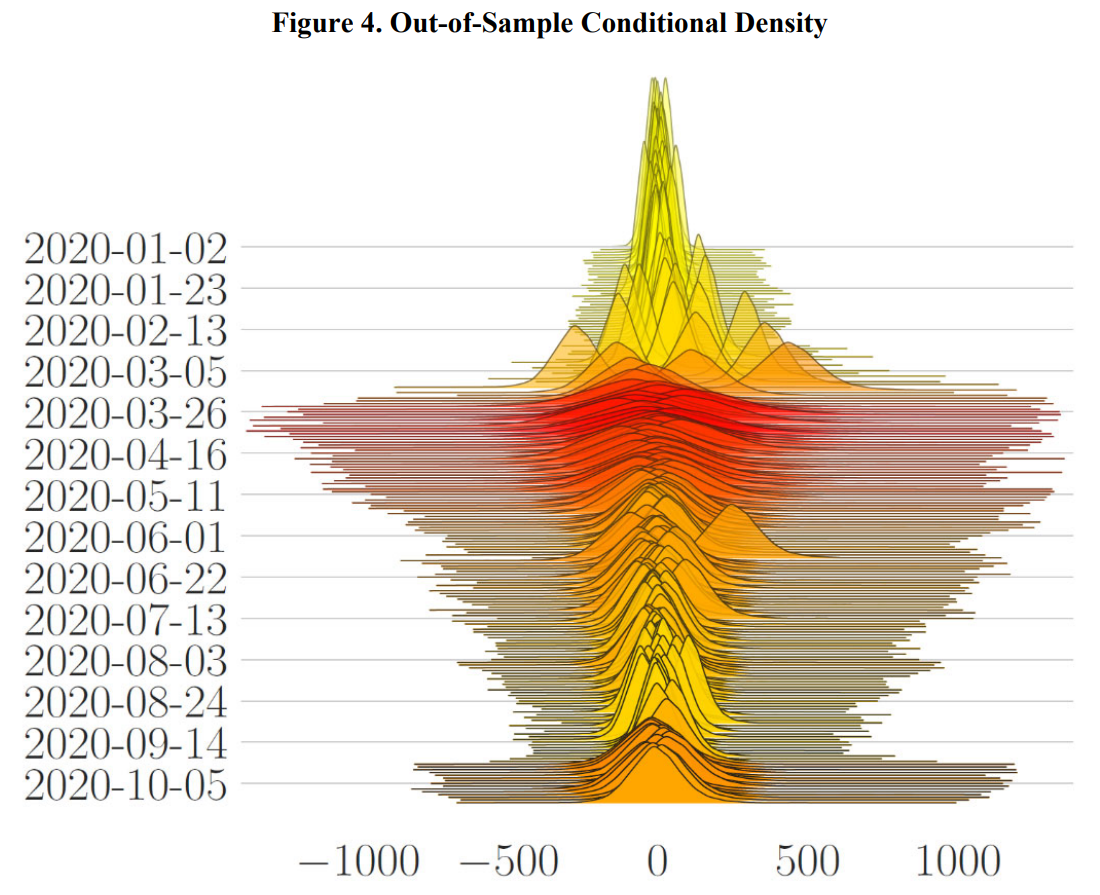
\includegraphics[width=0.75\paperwidth]{../static/course_3_img/var_fxi_conditional_density.PNG}}
  \hspace*{15pt}\hbox{\scriptsize Credit:\thinspace{\scriptsize\itshape Lafarguette and Veyrune (2021)}}          
\end{frame}

\begin{frame}
  \frametitle{Application: MXN/USD Fan Chart}
  \makebox[\linewidth]{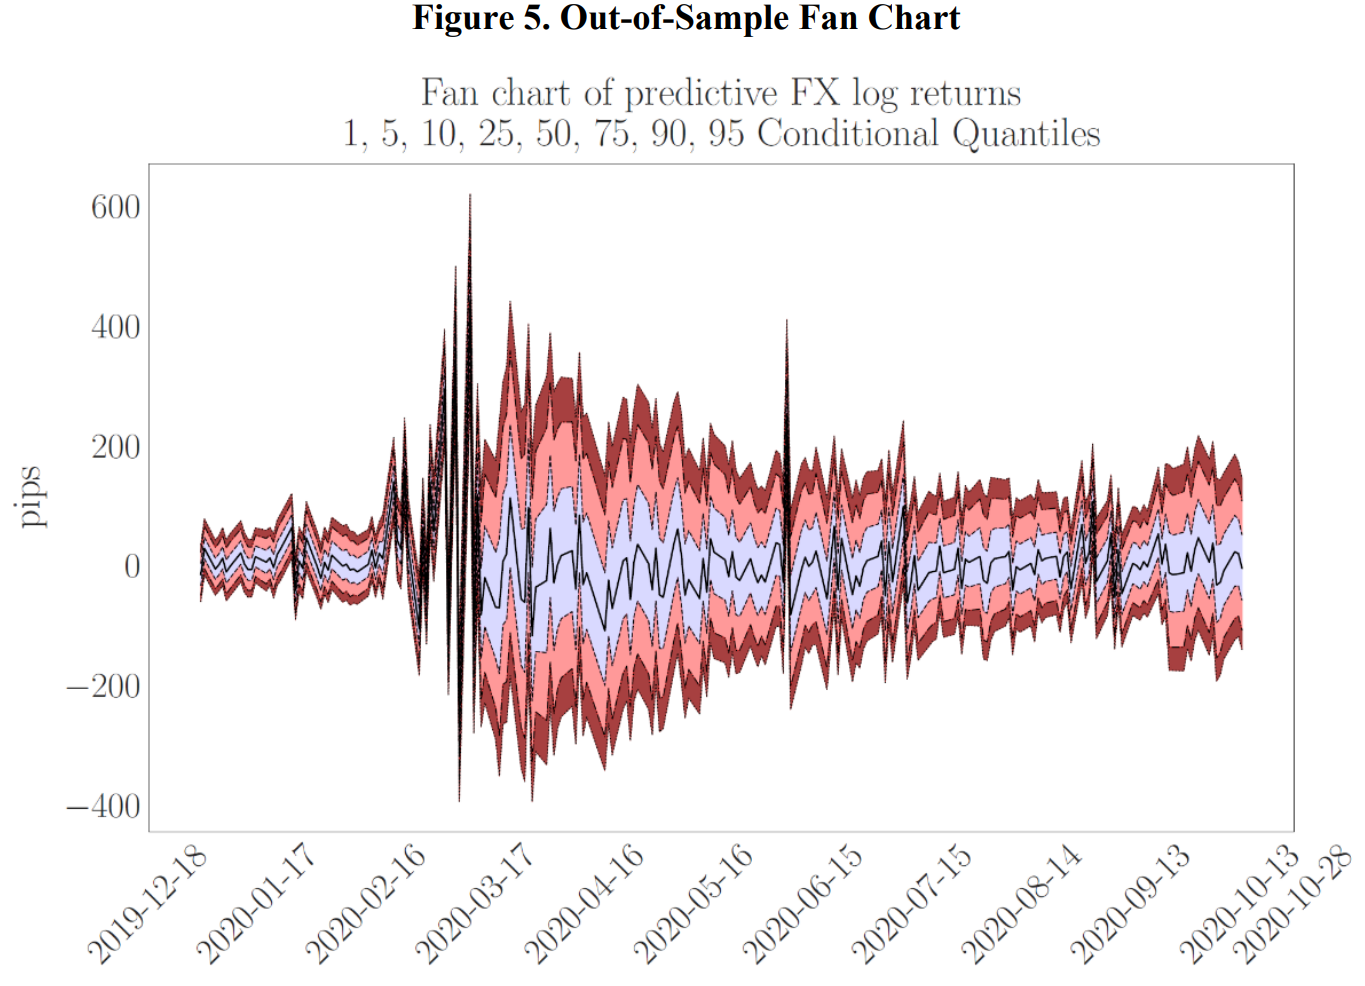
\includegraphics[width=0.85\paperwidth]{../static/course_3_img/var_fxi_fan_chart.PNG}}
  \hspace*{15pt}\hbox{\scriptsize Credit:\thinspace{\scriptsize\itshape Lafarguette and Veyrune (2021)}}          
\end{frame}

\begin{frame}
  \frametitle{Application: MXN/USD Intervention Rule}
  \makebox[\linewidth]{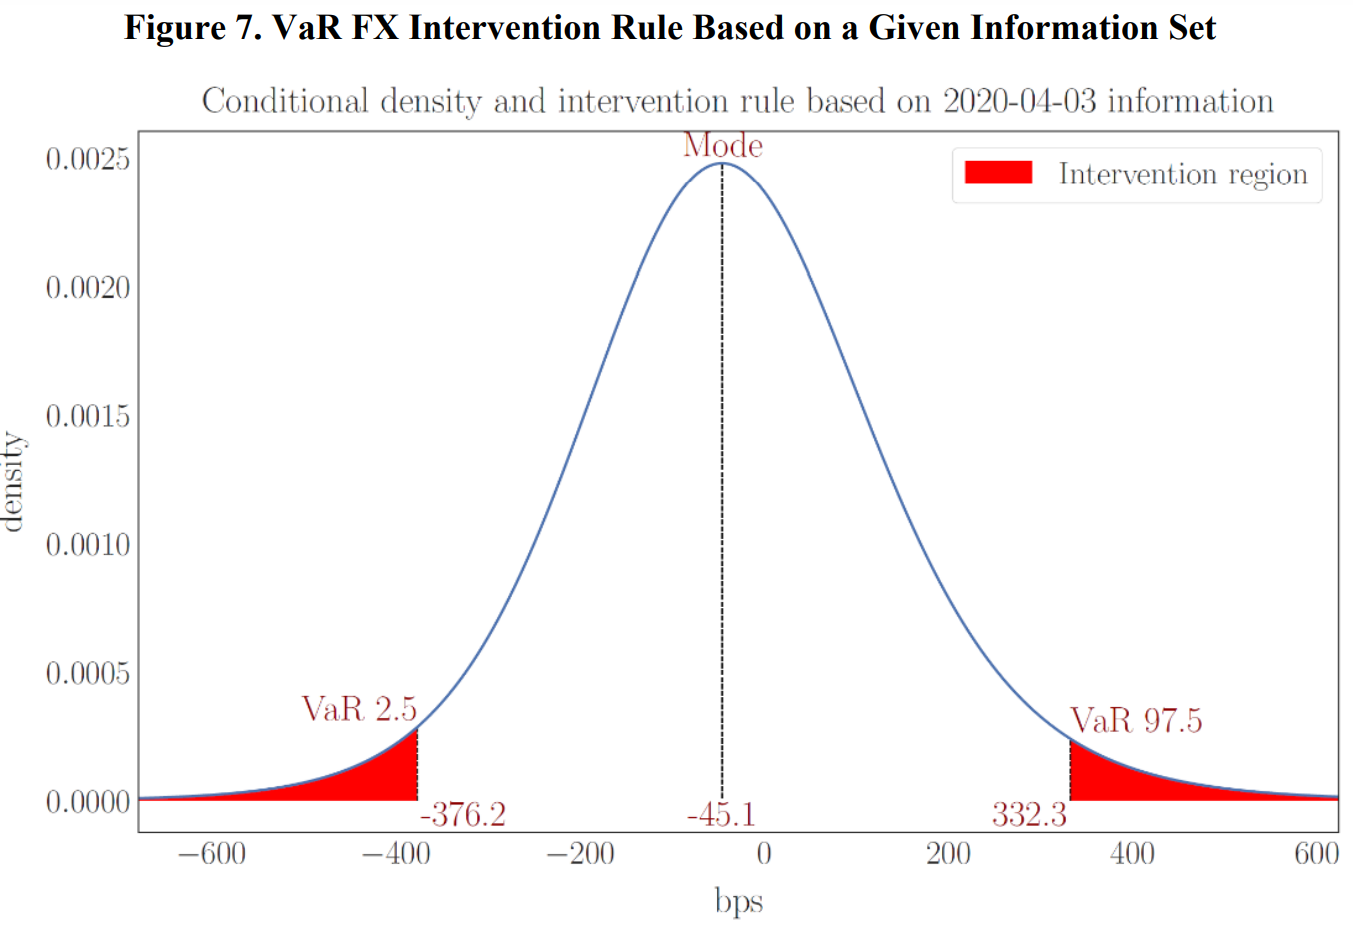
\includegraphics[width=0.85\paperwidth]{../static/course_3_img/var_fxi_intervention_rule.PNG}}
  \hspace*{15pt}\hbox{\scriptsize Credit:\thinspace{\scriptsize\itshape Lafarguette and Veyrune (2021)}}          
\end{frame}

\section{Distributional Forecasts and Prediction Intervals}
\begin{frame}{From Point Forecasts to Distributional Forecasts}

  \begin{wideitemize}
    \item A forecast $\hat{y}_{T+h|T}$ is (usually) the mean of the conditional distribution: $Y_{T+h} | Y_1, \dots Y_T$
    \item Most models produces Gaussian distributed forecast
    \item Because models assumes Gaussian residuals: remember that the residuals are the stochastic components that are determining the distribution of both the estimators and the forecasts
    \item The forecast distribution describes the probability to forecast any future value
  \end{wideitemize}

  %TODO: add a chart
    
\end{frame}


\begin{frame}{Distributional Forecasts}

  Assuming the \textbf{residuals are uncorrelated} with variance $\sigma^2$, and with an estimate $\hat{\sigma^2}$

  \begin{alertblock}{Model Typology}
    \begin{wideitemize}
      \item \textbf{Mean:} $Y_{T+h|T} = \mathcal{N}(\overline{Y}, (1+\frac{1}{T})\hat{\sigma^2})$
      \item \textbf{Naive:} $Y_{T+h|T} = \mathcal{N}(Y_T, h\hat{\sigma^2})$
      \item \textbf{Seasonal Naive:} $Y_{T+h|T} = \mathcal{N}(Y_{T+h-m(k+1)}, (k+1)\hat{\sigma^2})$
      \item \textbf{Drift:} $Y_{T+h|T} = \mathcal{N}(Y_{T} +\frac{h}{T-1}(Y_T - Y_1), h\frac{T+h}{T}\hat{\sigma^2})$
    \end{wideitemize}
  \end{alertblock}

\medskip

\begin{wideitemize}
  \item where $k$ is the integer part of $\frac{h-1}{m}$
  \item Note that when $h=1$ and $T$ is large, these all give the same approximate variance $\hat{\sigma^2}$
\end{wideitemize}

\end{frame}



\begin{frame}{Prediction Intervals}
  \begin{block}{Definition}
      A prediction interval gives \textbf{a region} within which we expect $Y_{T+h}$ to lie with \textbf{a specified probability}
  \end{block}

\medskip
  
  \begin{wideitemize}
  \item Assuming that the forecasting errors are normally distributed, then a 95\% prediction interval is:
    \begin{equation*}
      Y_{T+h|T} \pm 1.96 \hat{\sigma_h}
    \end{equation*}
  \item where $\hat{\sigma_h}$ is the standard deviation of the h-step distribution
  \item when $h=1$, $\hat{\sigma_h}$ can be estimated from the residuals  
  \end{wideitemize}  
\end{frame}


\begin{frame}
  \frametitle{Prediction Interval Fit}
     \makebox[\linewidth]{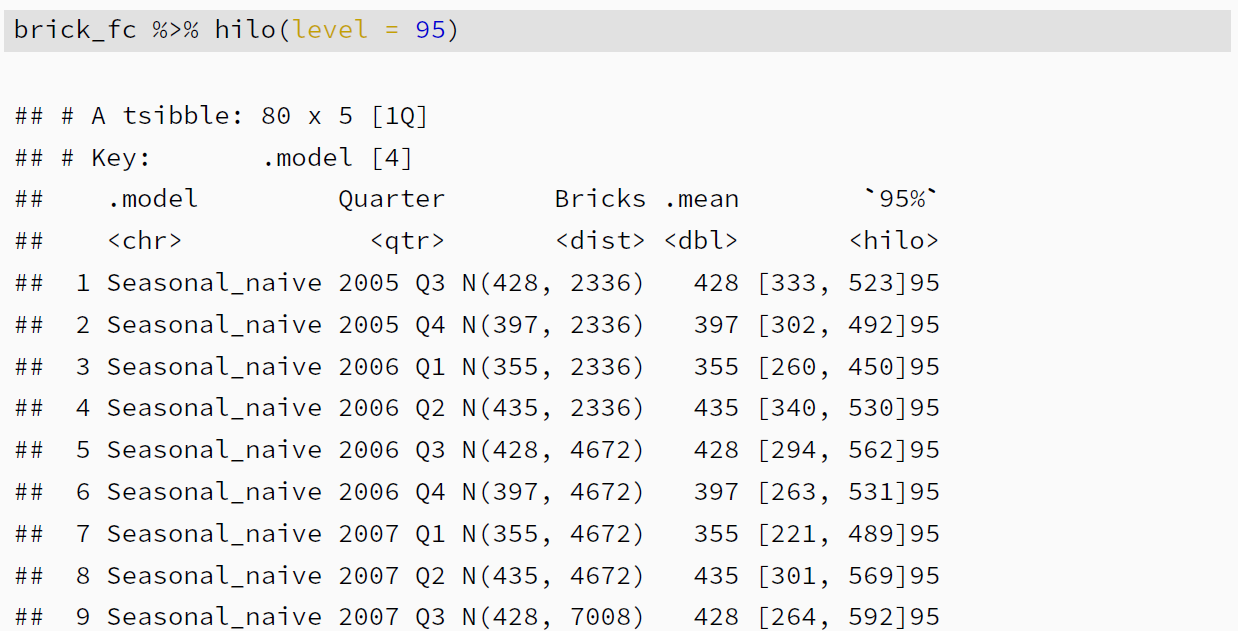
\includegraphics[width=0.95\paperwidth]{../static/course_3_img/prediction_interval.PNG}}  
\end{frame}


\begin{frame}{Why Prediction Intervals Matter}
  \begin{wideitemize}
    \item \textbf{Point forecasts are often useless without a measure of uncertainty} (such as prediction intervals)
    \item Prediction intervals require a \textbf{stochastic model} (with random errors, etc.)
    \item For most models, prediction intervals get wider as the forecast horizon increases
    \item The degree of confidence (the probability) impacts the width of the prediction interval
    \item Usually too narrow due to unaccounted uncertainty: pay attention
  \end{wideitemize}  
\end{frame}


\begin{frame}
  \frametitle{Difference between Confidence Interval and Prediction Interval}
  \begin{wideitemize}


 \item A confidence interval informs about where the true parameter of a model can be
   \begin{itemize}
     \item \textbf{Confidence interval quantifies the uncertainty about the model}, or the distance between the model and reality
     \item Confidence interval are associated with a wide range of parameters, values, etc.
     \item They inform about how the model represents well the reality
     \item Wide confidence intervals are associated with a less accurate model, and/or a very volatile model
   \end{itemize}

    
  \item The prediction interval predicts in what range a future individual observation will fall
    \begin{itemize}
      \item \textbf{Prediction interval quantifies the uncertainty about the future}, or the distance between today and the future
      \item Prediction interval are not about the parameters of the model, but about the dependent variable ($y_t$)
      \item The problem is that prediction intervals tend to neglect the uncertainty about the parameters used to generate the forecasts...
    \end{itemize}   
  \end{wideitemize}
  
\end{frame}


\begin{frame}
  \frametitle{Difference between Confidence Interval and Prediction Interval}
     \makebox[\linewidth]{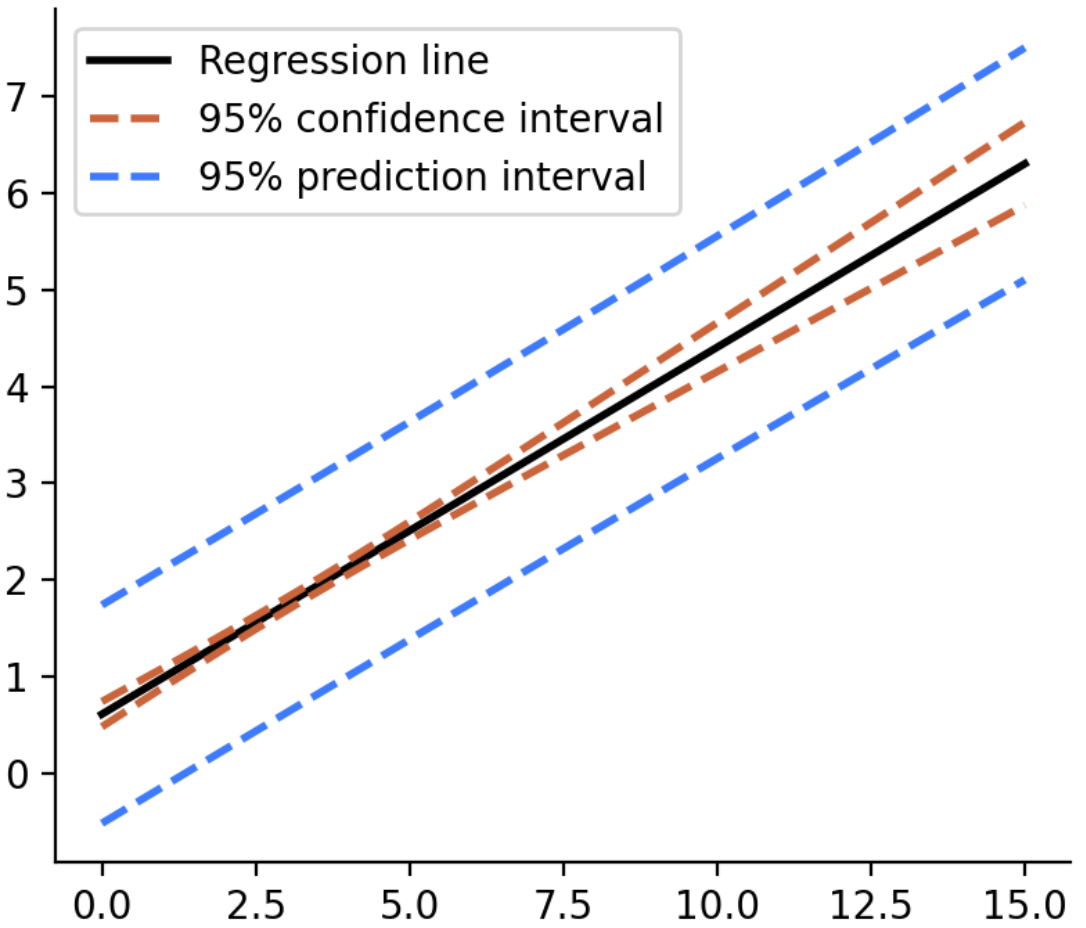
\includegraphics[width=0.75\paperwidth]{../static/course_3_img/pi_ci.png}}  
\end{frame}


\section{Evaluating Forecast Accuracy}

\begin{frame}{Fitting and Forecasting}

  \begin{alertblock}{Be careful}
    \textbf{A model that fits the data well (in sample) might not necessarily forecast well}
  \end{alertblock}

  \medskip
  
  \begin{wideitemize}
    \item A perfect in-sample fit can always be obtained by using a model with with enough parameters
    \item Over-fitting a model to data is just as bad as failing to identify a systematic pattern in the data
    \item Need to split the model between 
    \item The test set must no be used to \emph{any} aspect of model development or calculation of forecasts
    \item Forecast accuracy is only based on the test set
  \end{wideitemize}  
\end{frame}

\begin{frame}
  \frametitle{Train and Test Set}
     \makebox[\linewidth]{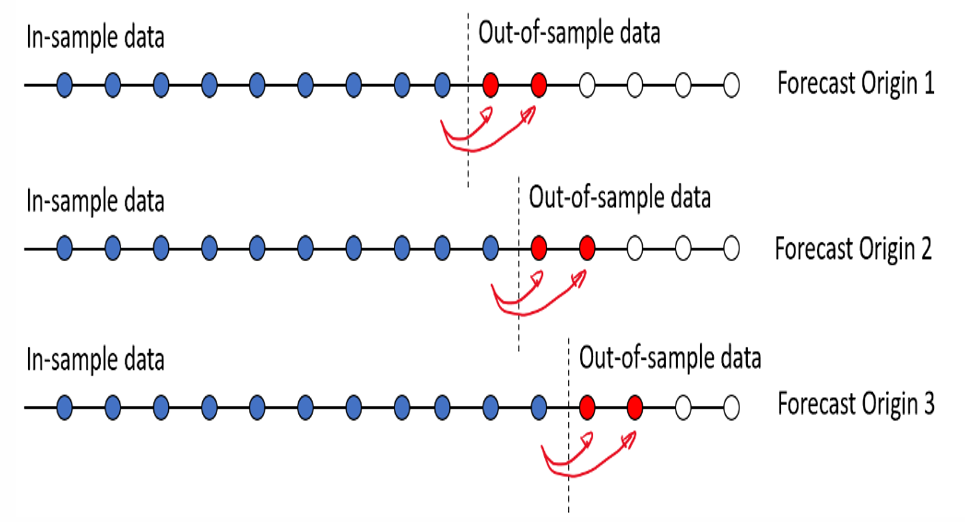
\includegraphics[width=0.95\paperwidth]{../static/course_3_img/in_sample_out_sample.PNG}}  
\end{frame}

\begin{frame}
  \frametitle{Underfit, Optimal, Overfit}
     \makebox[\linewidth]{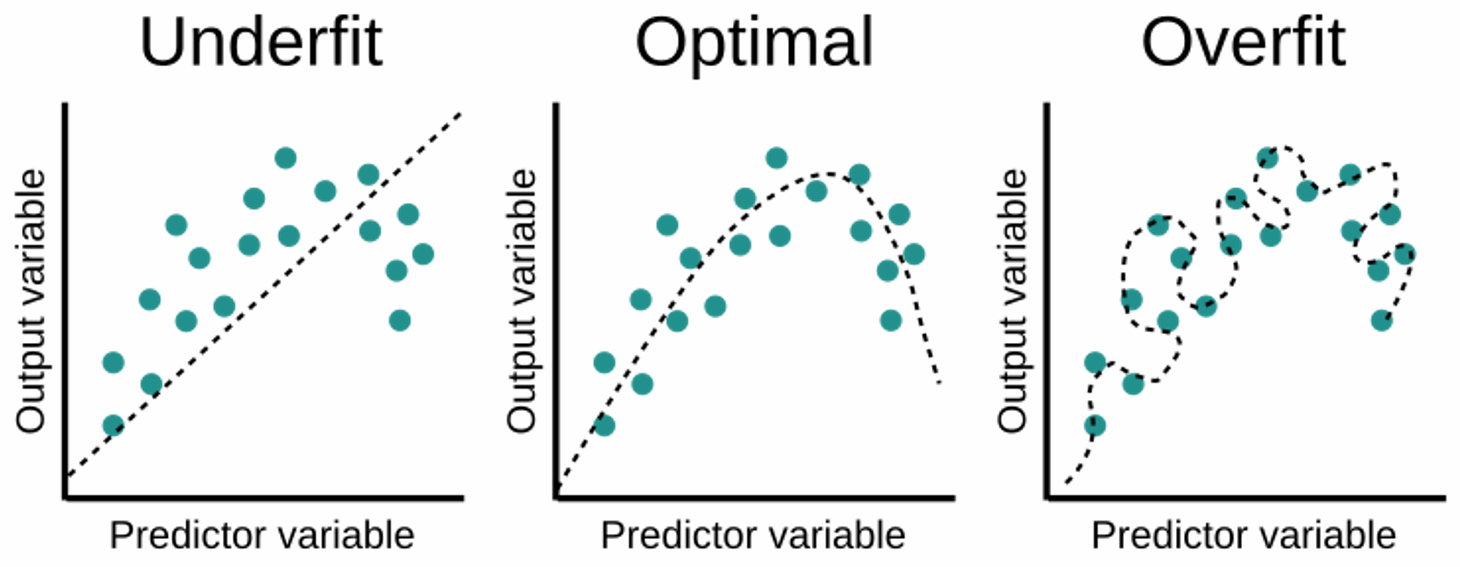
\includegraphics[width=0.95\paperwidth]{../static/course_3_img/overfit_underfit.PNG}}  
\end{frame}

\begin{frame}{Forecast Errors}

  \begin{block}{Definition: Forecast Errors}
    A forecast error is the difference between an observed value and its forecast

    \begin{equation*}
      e_{T+h} = y_{T+h} - \hat{y}_{T+h}|Y_T, \dots, Y_1
    \end{equation*}
  \end{block}

\medskip
  
\begin{wideitemize}
    \item The conditional set $Y_T, \dots, Y_1$ should only be taken from the training dataset
    \item The true value $y_{T+h}$ is taken from the test set
    \item Unlike residuals, forecast errors on the test involve multi-step forecasts
    \item These are the \textbf{true} forecast error, as the test data is not used to compute $\hat{y}_{T+h}$
  \end{wideitemize}
  
\end{frame}

\begin{frame}
  \frametitle{Example: Forecasting Beer Production}
     \makebox[\linewidth]{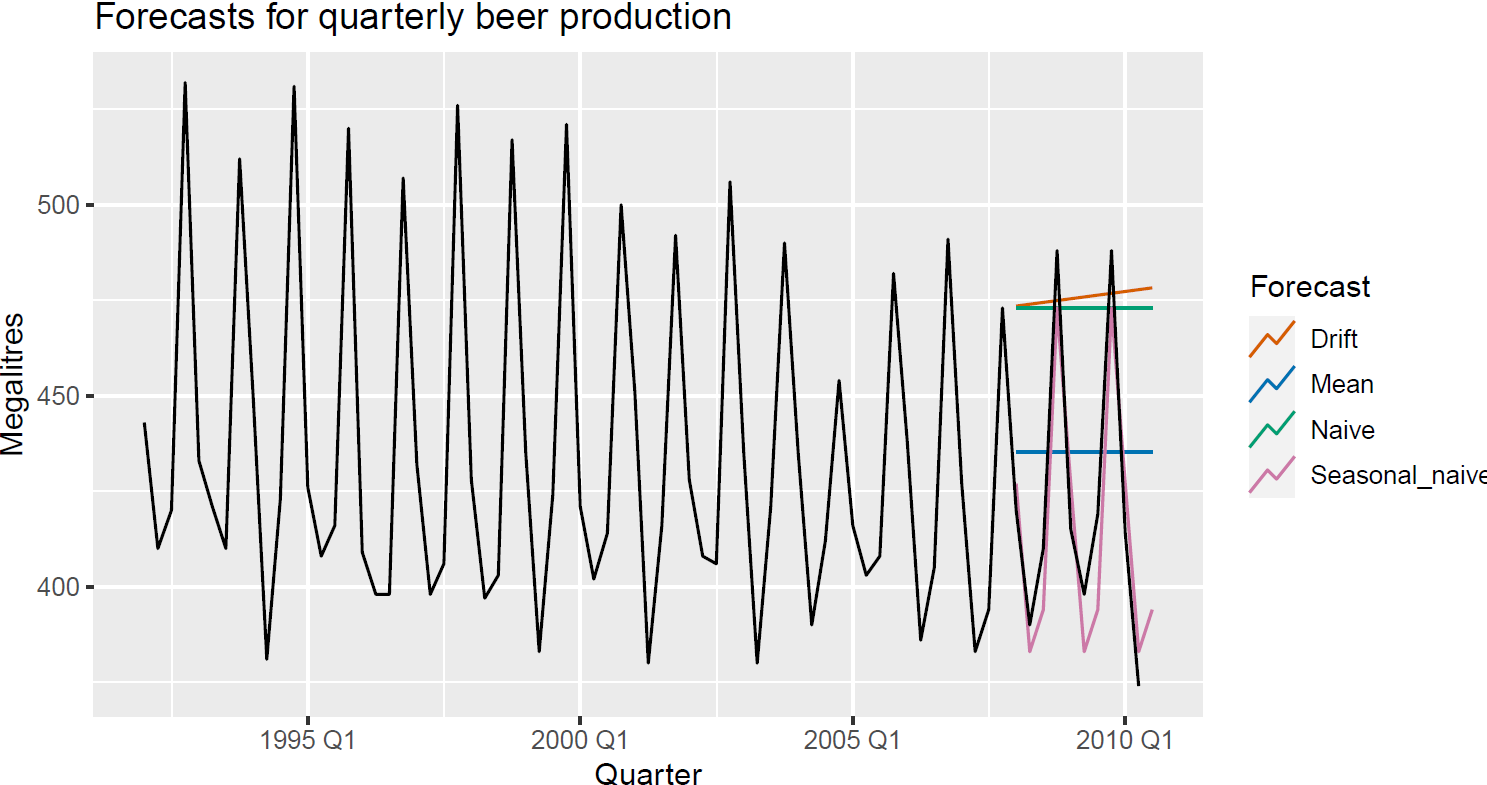
\includegraphics[width=0.95\paperwidth]{../static/course_3_img/beer_forecast.PNG}}  
\end{frame}

\begin{frame}{Measures of Forecast Accuracy}

  \begin{alertblock}{Main Metrics}
    \begin{wideitemize}
    \item \textbf{MAE}: mean absolute errors $\frac{1}{S}\sum_{s \in S} |e_{s, T+h}|$
    \item \textbf{MSE}: mean squared errors $\frac{1}{S}\sum_{s \in S} (e_{s, T+h})^2$
    \item \textbf{MAPE}: mean absolute percentage errors $\frac{1}{S}100*\sum_{s \in S} \frac{|e_{s, T+h}|}{|y_{s, t+h}|}$
    \item \textbf{RMSE}: root mean squared errors: $\sqrt{\frac{1}{S}\sum_{s \in S} (e_{s, T+h})^2}$
    \end{wideitemize}
  \end{alertblock}

  With:\\
  
  \begin{itemize}
  \item $y_{T+h}$: T+h observation, h being the horizon (h = 1, 2, ..., H)
  \item $\hat{y}_{T+h|T}$: the forecast based on data up to time $T$
  \item $e_{T+h} = y_{T+h} - \hat{y}_{T+h|T}$: The forecast errors
  \item $S$ is the testing sample
  \end{itemize}
\end{frame}

\begin{frame}{Scaling}  
  \begin{wideitemize}
  \item MAE, MSE and RMSE are all \textbf{scale dependent}
  \item MAPE is scale independent but is only sensible if $y_t >> 0 \qquad \forall \ t$
  \item \textbf{Most commonly used: Time Cross-Validation with the lowest RMSE}
  \end{wideitemize}  
\end{frame}


\begin{frame}
  \frametitle{Time Series Cross-Validation}
     \makebox[\linewidth]{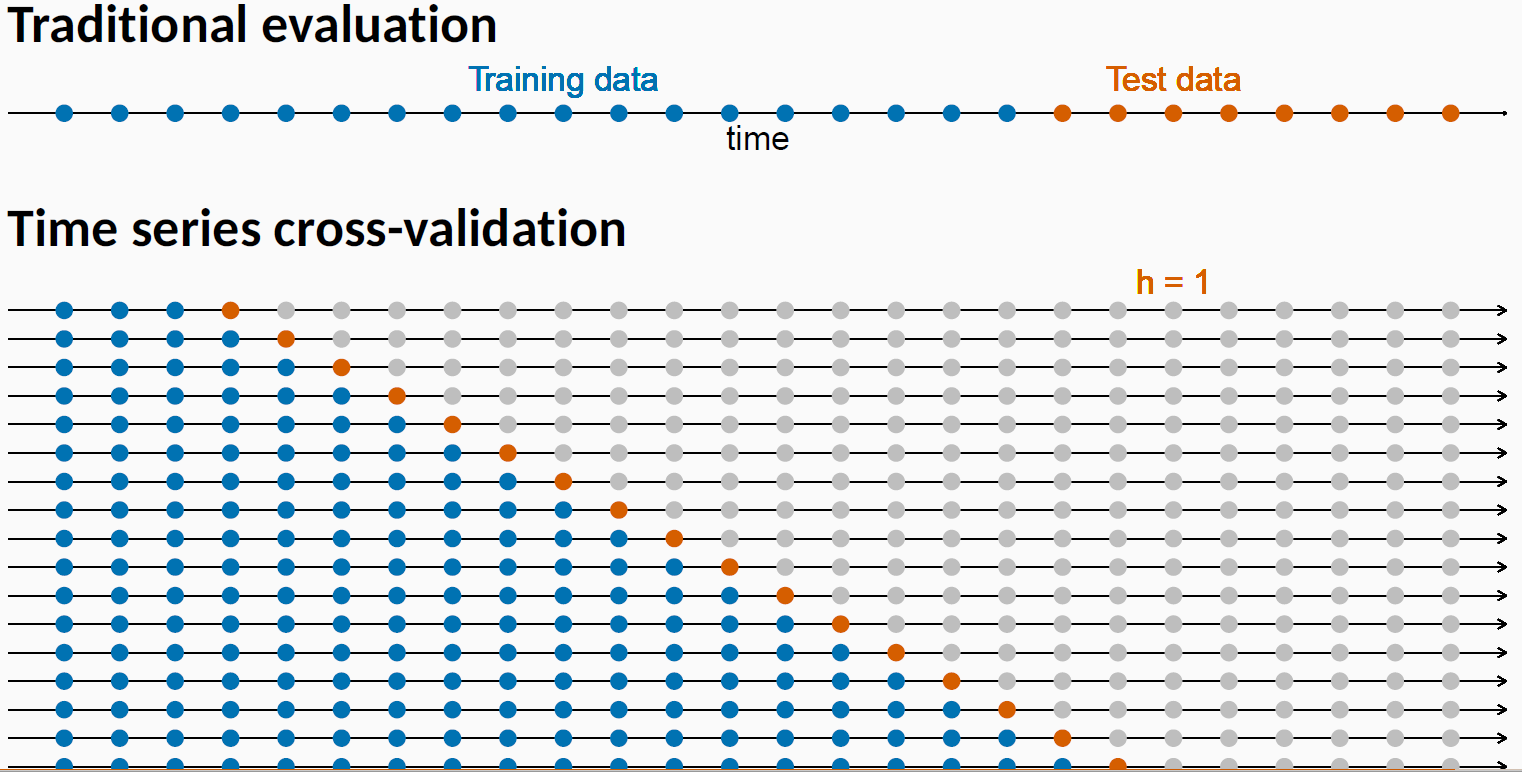
\includegraphics[width=0.95\paperwidth]{../static/course_3_img/time_series_cv_1.PNG}}  
  \end{frame}

\begin{frame}
  \frametitle{Time Series Cross-Validation}
     \makebox[\linewidth]{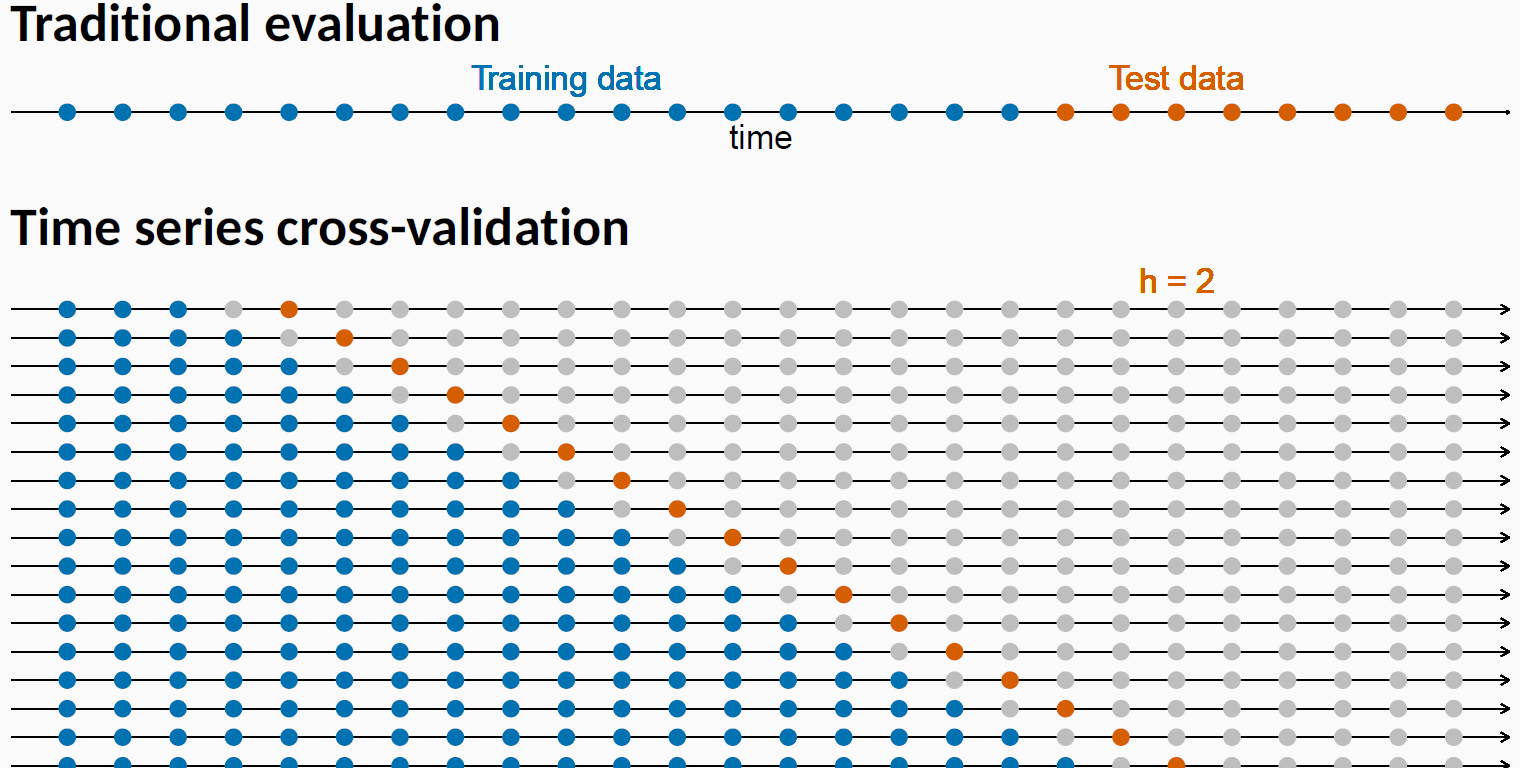
\includegraphics[width=0.95\paperwidth]{../static/course_3_img/time_series_cv_2.PNG}}  
  \end{frame}

\begin{frame}
  \frametitle{Time Series Cross-Validation}
     \makebox[\linewidth]{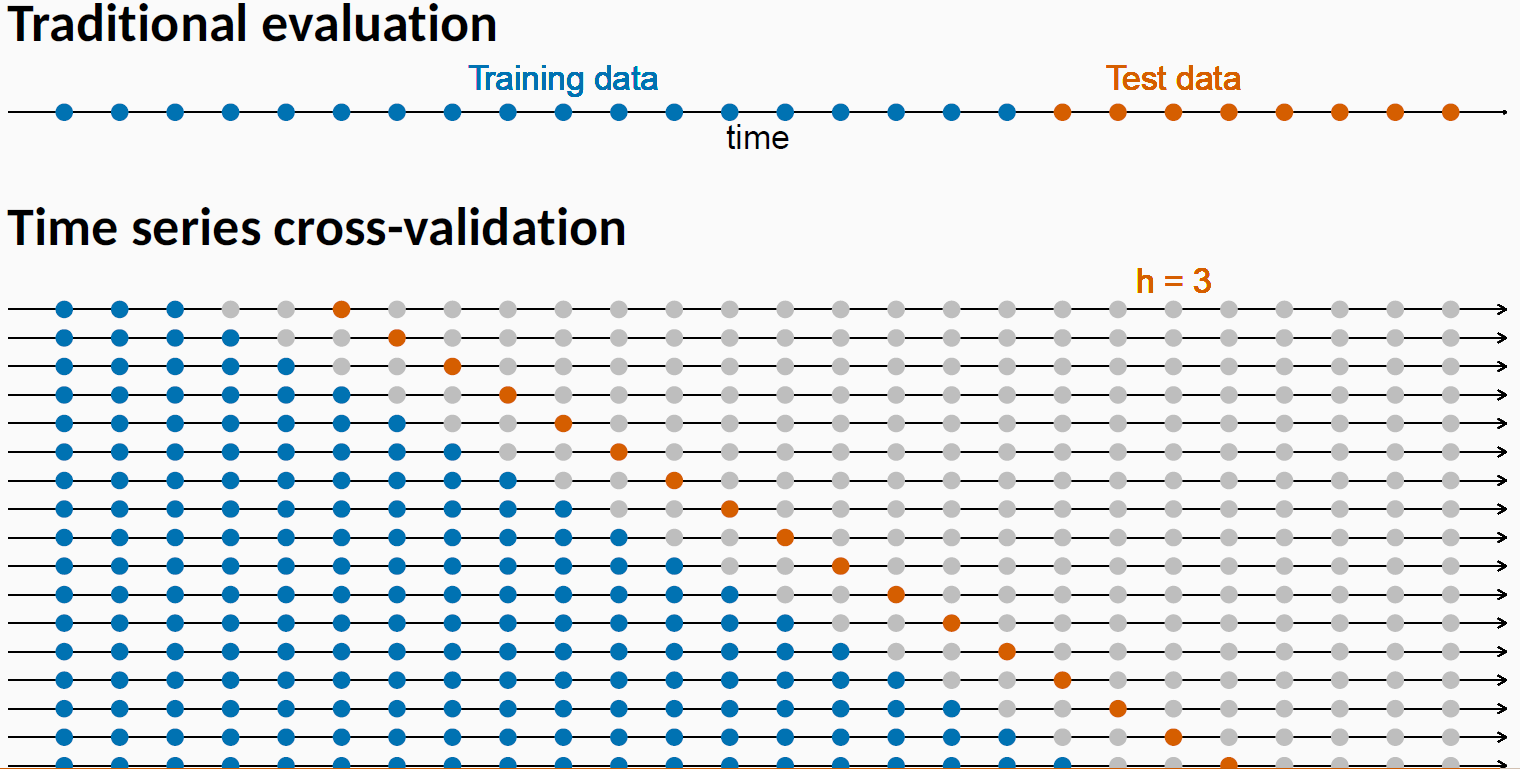
\includegraphics[width=0.95\paperwidth]{../static/course_3_img/time_series_cv_3.PNG}}  
  \end{frame}

\begin{frame}
  \frametitle{Time Series Cross-Validation}
     \makebox[\linewidth]{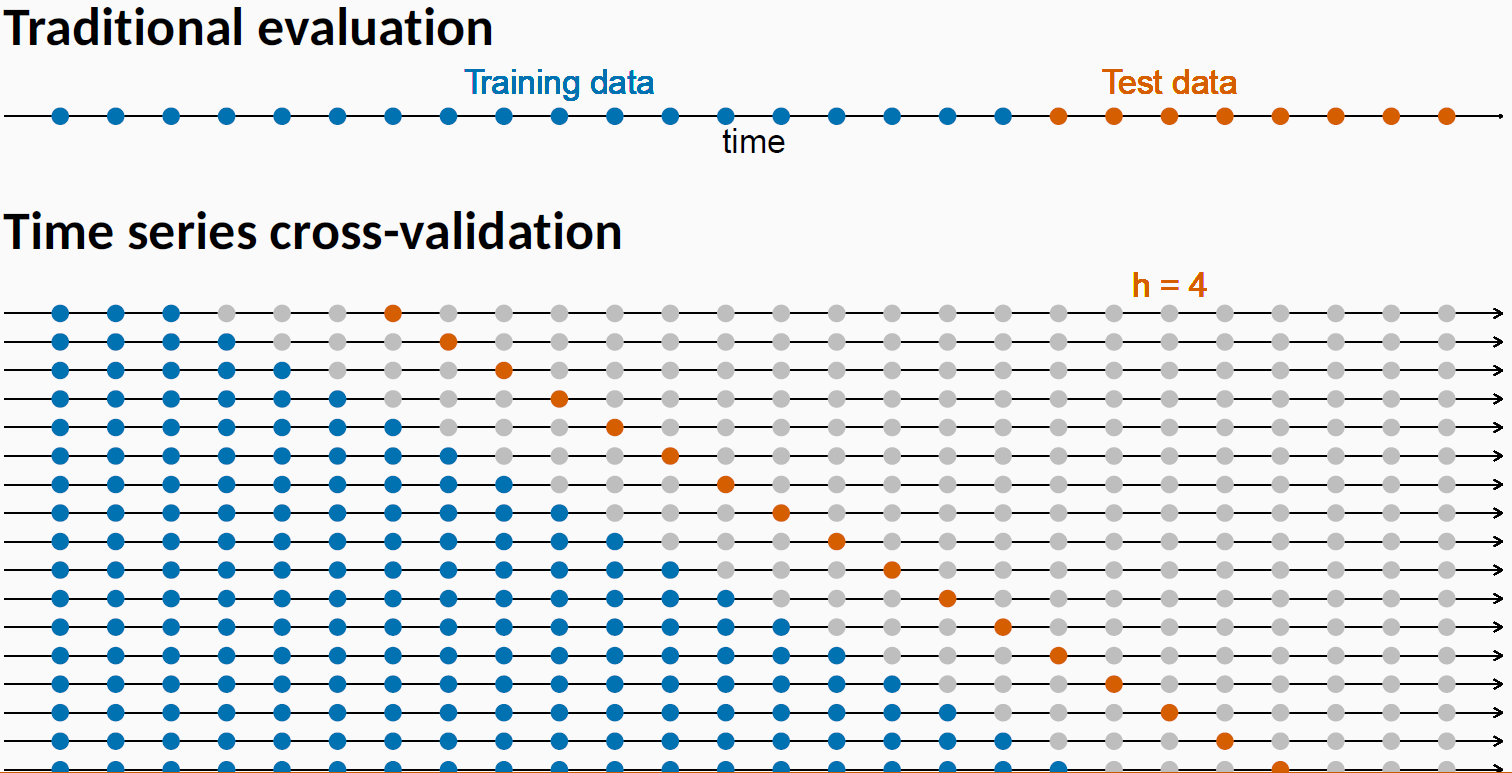
\includegraphics[width=0.95\paperwidth]{../static/course_3_img/time_series_cv_4.PNG}}  
  \end{frame}

\begin{frame}
  \frametitle{Time Series Cross-Validation}
     \makebox[\linewidth]{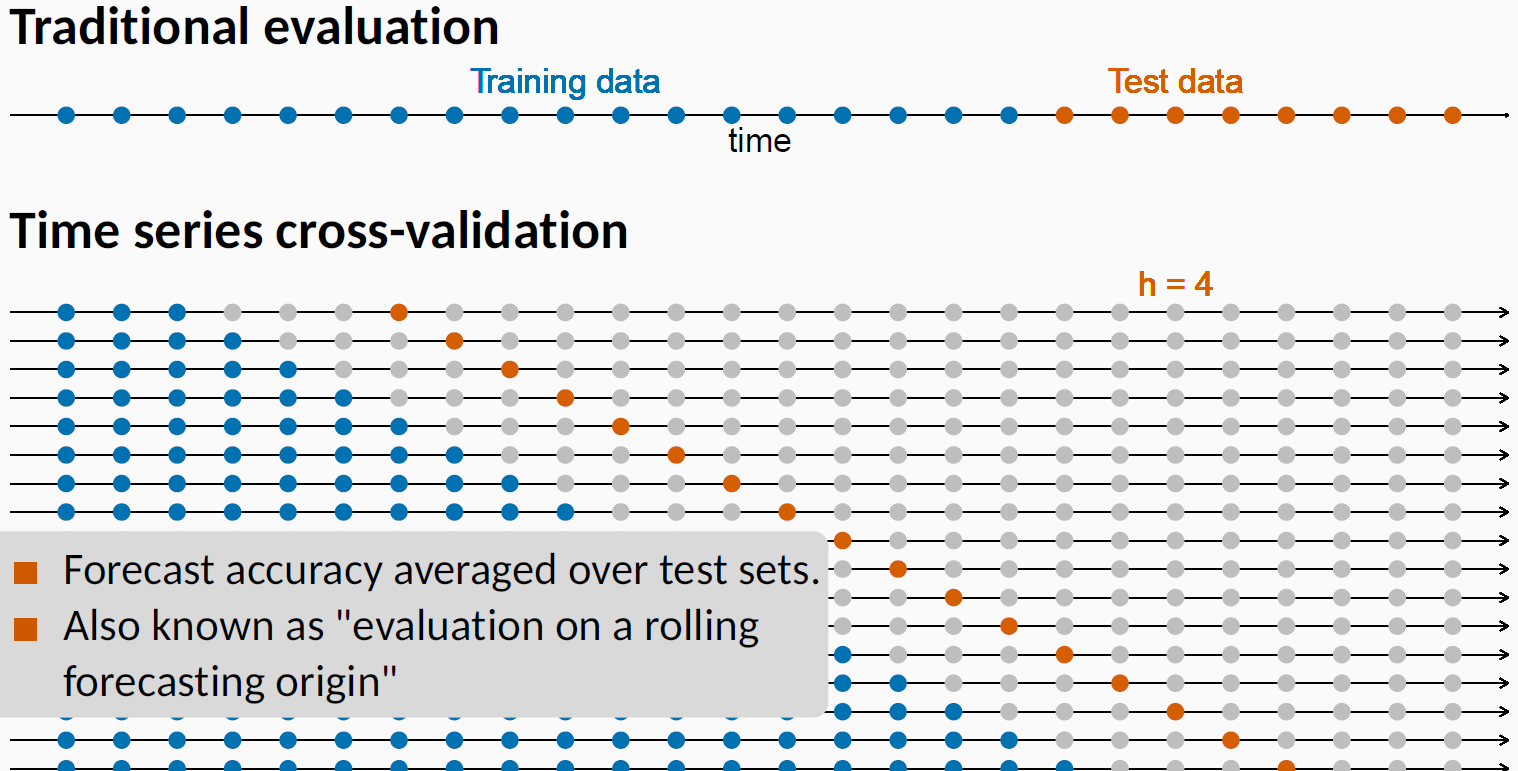
\includegraphics[width=0.95\paperwidth]{../static/course_3_img/time_series_cv_5.PNG}}  
  \end{frame}


    \begin{frame}
      \frametitle{Framework RMSE Output}
  \makebox[\linewidth]{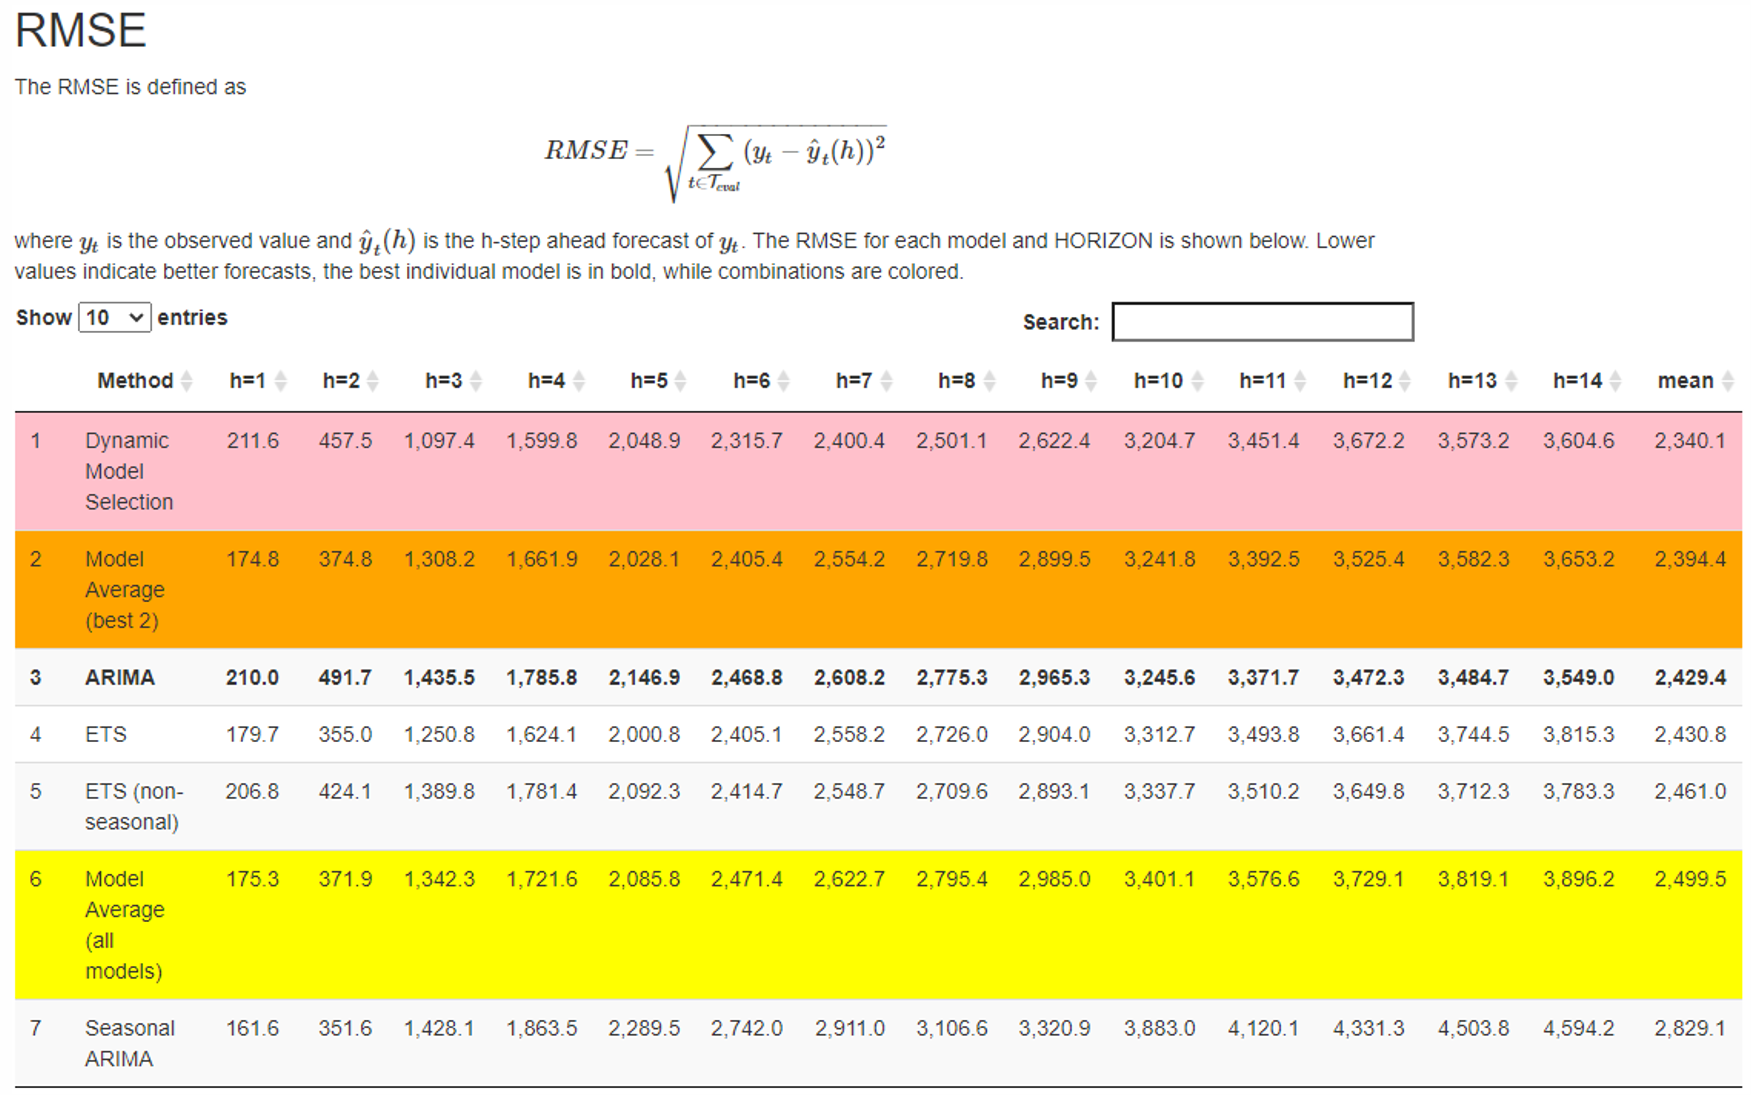
\includegraphics[width=0.85\paperwidth]{../static/course_3_img/rmse_output.PNG}}
  \hspace*{15pt}\hbox{\scriptsize Credit:\thinspace{\scriptsize\itshape IMF Framework}}      
    \end{frame}


    \begin{frame}
      \frametitle{Nemenyi Test}

      \begin{wideitemize}
        \item We can rank the model by RMSE (or another metric), but are the RMSE significantly different? 
        \item Maybe Model 1 can have a lower RMSE than Model 2, but the difference in RMSE is non-significant
        \item In which case, we could pool the two models together
        \item Use a non-parametric test to test the hypothesis of equal RMSE, with the test statistic:
          \begin{equation*}
            r_{\alpha, K, N} \approx \frac{q_{\alpha, K}}{\sqrt{2}} \sqrt{\frac{K (K+1)}{6N}}
          \end{equation*}
      \end{wideitemize}      
    \end{frame}

    \begin{frame}
      \frametitle{Nemenyi Test in Practice}
  \makebox[\linewidth]{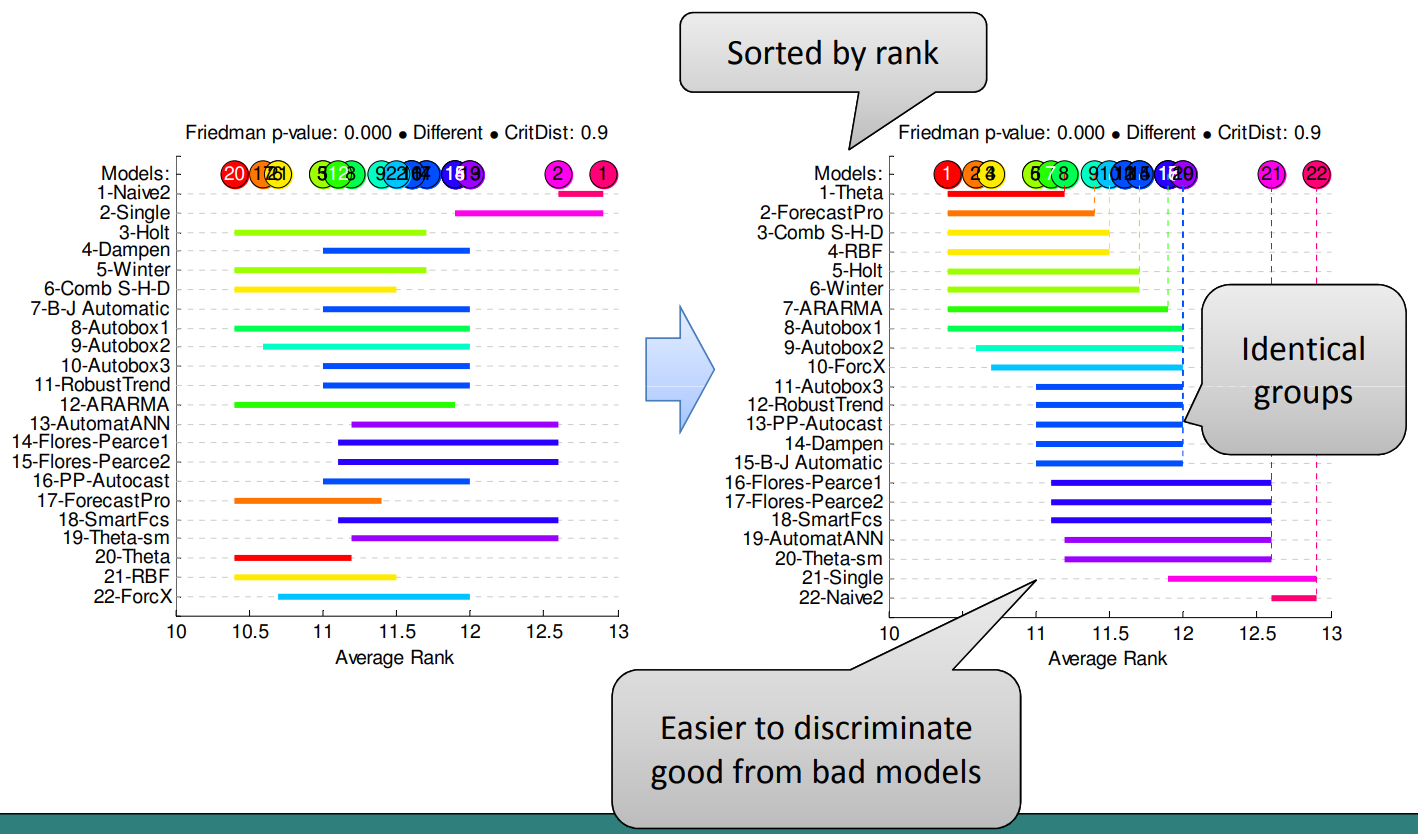
\includegraphics[width=0.85\paperwidth]{../static/course_3_img/nemenyi_test.PNG}}
  \hspace*{15pt}\hbox{\scriptsize Credit:\thinspace{\scriptsize\itshape Nikolaos Kourentzes}}      
    \end{frame}

    
    
\section{Model Combination and Selection}

\begin{frame}
  \frametitle{Combination of Models}

  \begin{wideitemize}
    \item Combining model provides a more reliable forecast, overcoming the risk of relying on a single model
    \item Estimate all the models, determine the cross-validated errors
    \item Define a pool of "good" models and reject the other models, based on their out of sample performance. Define a \textbf{rejection threshold} to determine the "bad" models, based on the distribution of the RMSE
      \begin{equation*}
        \text{Threshold} = Q(0.75) + 1.5*\text{IQR}
      \end{equation*}
      \begin{itemize}
      \item Where $Q(0.75)$ is the 75th quantile of the RMSE distribution and IQR the interquantile range ($Q(0.75) - Q(0.25)$)
      \end{itemize}
    \item Then, weight each forecast of the eligible model by the relative performance of their model, the best models having the highest weight
    \item Advantage: optimize performance and reduce modeling risks, doesn’t rely on a single model: model diversity is advantageous    
  \end{wideitemize}
  
\end{frame}

\begin{frame}
  \frametitle{Dynamic Model Selection: Principles}

  \begin{wideitemize}
    \item Some models are better for modelling long-term dynamics, while others are better are short-term dynamics 
    \item Time-varying volatility matters. As volatility increases, models focusing on the short term have an advantage
    \item Dynamically account for changes in the behaviour of the time series:
      \begin{itemize}
      \item Combining high performing forecasts
      \item Selecting a well performing forecast based on local performance
      \end{itemize}
  \end{wideitemize}  
\end{frame}


\begin{frame}
  \frametitle{Dynamic Model Selection: Implementation}

  \begin{wideitemize}
  \item \textbf{Combining high-performance forecasts:}
    \begin{itemize}
    \item Compute unweighted average of forecasts. Although it seems better to estimate “optimal” weights, weights estimation introduces additional uncertainty  
    \end{itemize}
  \item Selecting a well performing forecast based on \textbf{recent performance}
    \begin{itemize}
    \item \textbf{Rolling performance of the previous week} to select the forecast for the next origin. 
    \end{itemize}
    
  \item Consider ETStrig, ARIMAtrig, ARIMA stoch, and TBATS comp. All these models capture information differently
    \begin{itemize}
    \item \textbf{Model diversity is advantageous} both for selection and combination between forecasts
    \end{itemize}
  \end{wideitemize}  
\end{frame}

 \begin{frame}
 \frametitle{Out-of-Sample Performances via Rolling Origins}
  \makebox[\linewidth]{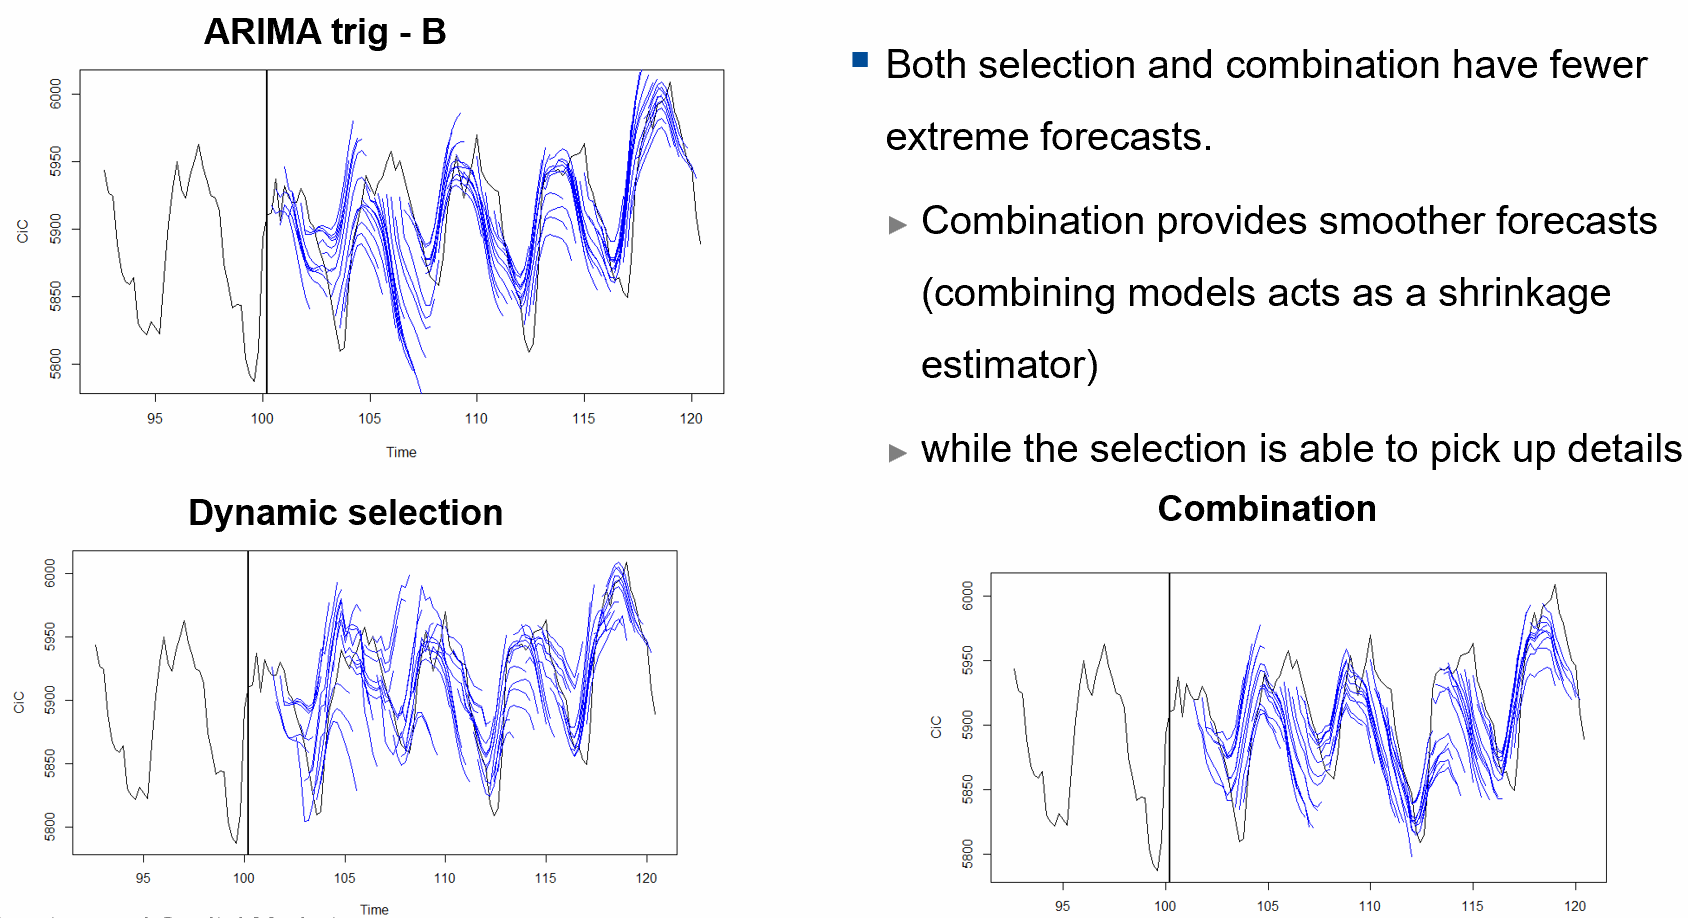
\includegraphics[width=0.75\paperwidth]{../static/course_3_img/arima_combination_selection.PNG}}
  \hspace*{15pt}\hbox{\scriptsize Credit:\thinspace{\scriptsize\itshape Author}}      
 \end{frame}


\section{Forecasts Reconciliation}
\begin{frame}
  \frametitle{Forecasts Reconciliation of the Autonomous Factors}

  Forecast the autonomous factors using a hierarchical modeling approach, with different models for each autonomous factor:\\
  \medskip

  \begin{wideitemize}
  \item Forecasting the sum of the autonomous factors separately\\
  \item Reconciling the forecasts using aggregation technics as described for instance in Hyndman, Rob J., et al. "Optimal combination forecasts for hierarchical time series." (2011)
  
  \item Use either OLS  or the “minT” approach: minimize the trace of the VarCov forecast matrix. Exploit the covariance among regressors to maximize the accuracy of the hierarchical forecasts    
  \end{wideitemize}   
\end{frame}

 \begin{frame}
 \frametitle{Reconciliation via Hierarchical Forecasts}
  \makebox[\linewidth]{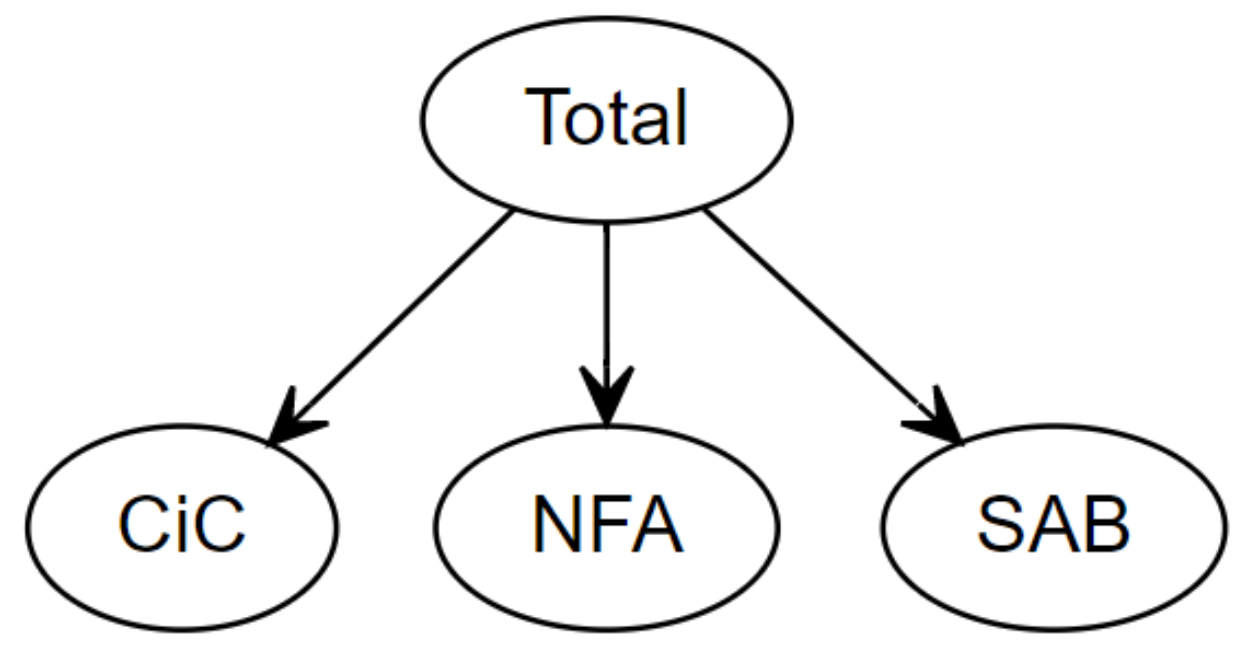
\includegraphics[width=0.75\paperwidth]{../static/course_3_img/hierarchical_forecasts.PNG}}
  \hspace*{15pt}\hbox{\scriptsize Credit:\thinspace{\scriptsize\itshape Author}}      
 \end{frame}


 \begin{frame}
 \frametitle{General Approach}

  \makebox[\linewidth]{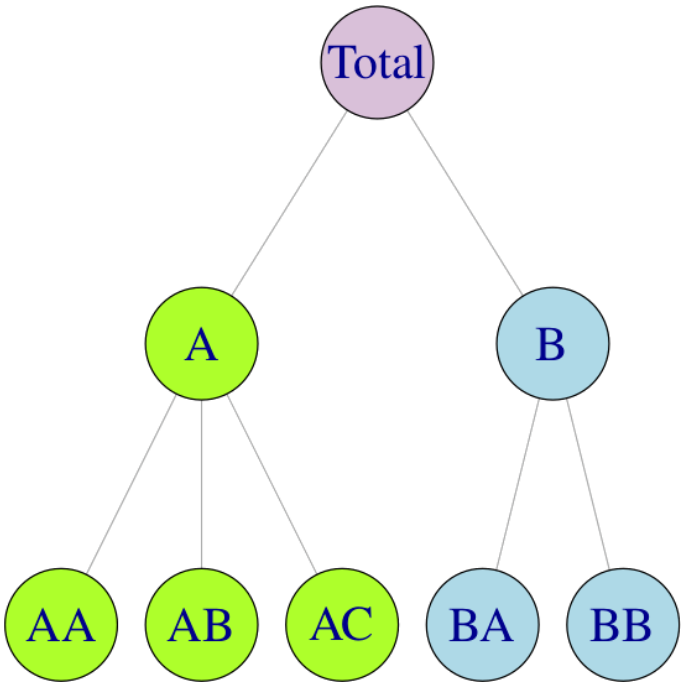
\includegraphics[width=0.5\paperwidth]{../static/course_3_img/hierarchical_forecasts_two_levels.PNG}}
  \hspace*{15pt}\hbox{\scriptsize Credit:\thinspace{\scriptsize\itshape https://otexts.com/fpp3/reconciliation.html}}      
 
 \end{frame}


 \begin{frame}
 \frametitle{Formalization}

 \begin{wideitemize}
 \item We can express the total (top level, $y_t$) via a summing matrix $S$ of the low level elements $y^L_t$
   \begin{equation*}
     y_t = S y^L_t
   \end{equation*}
 \item Then, we can express the whole system via a grouping matrix summing all the individual elements (also called base forecast $y^b_t$), so have a consistent approach irrespective of the level structure
   \begin{equation*}
     \tilde{y_t} = S*G*y^b_{h}
   \end{equation*}
 \end{wideitemize}

 \makebox[\linewidth]{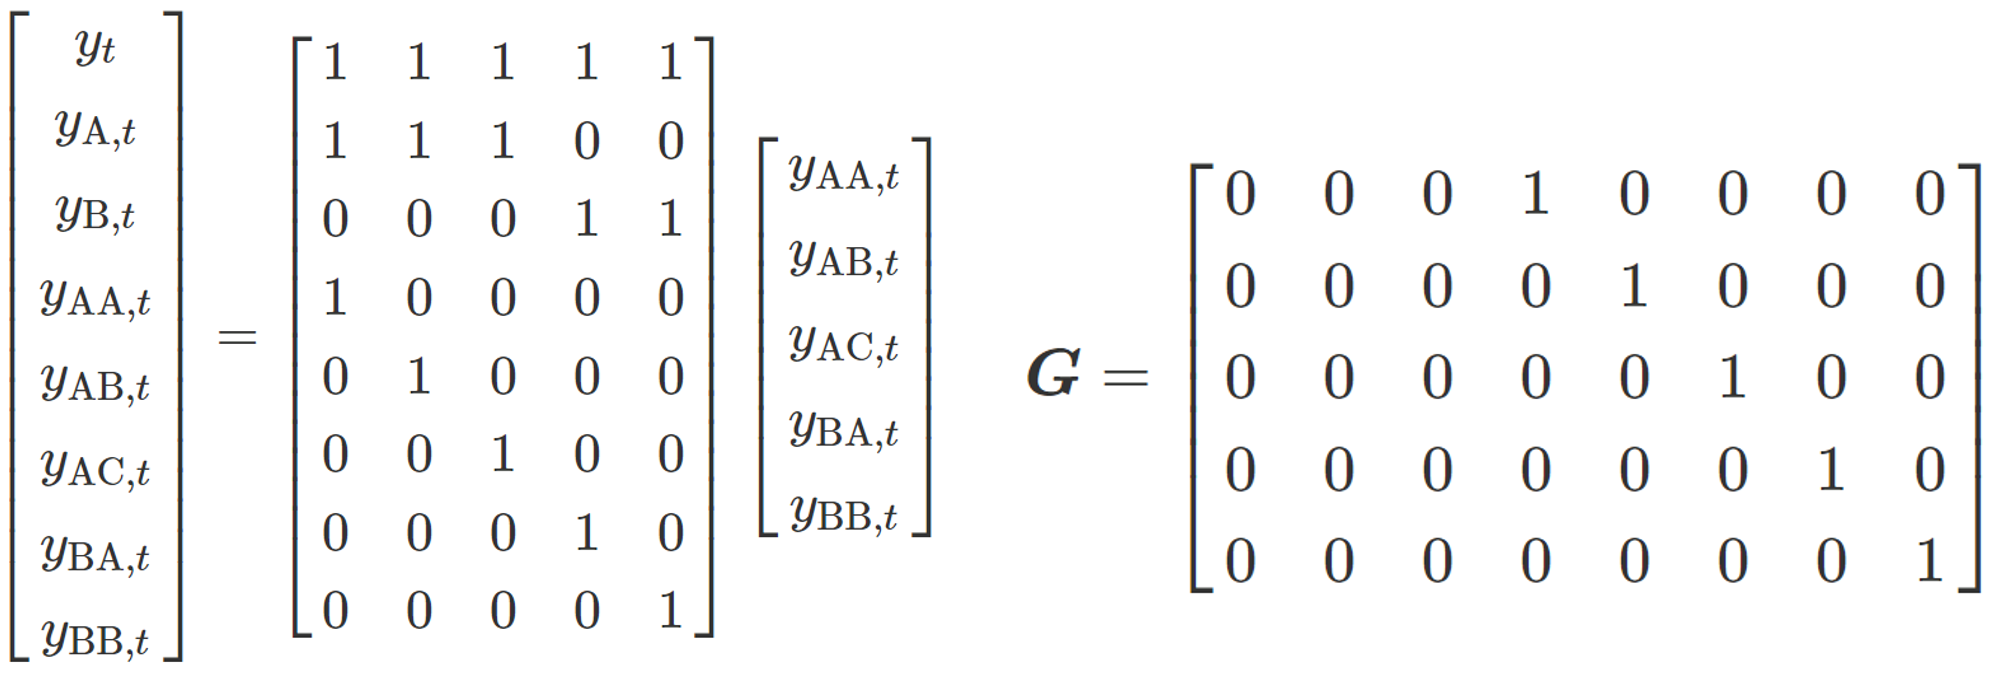
\includegraphics[height=0.25\paperheight]{../static/course_3_img/hierarchical_forecasts_two_matrices.PNG}}
 \hspace*{15pt}\hbox{\scriptsize Credit:\thinspace{\scriptsize\itshape otexts.com/fpp3/reconciliation.html}}      
 
 \end{frame}


 \begin{frame}
   \frametitle{The Min Trace Approach}
   \begin{block}{Forecasts Errors in a Hierarchical System}
     \begin{equation*}
       V_h = \mathbb{V}[y_{T+h} - \tilde{y_h}] = SGW_hG'S'
     \end{equation*}
   where $W_h = \mathbb{V}[y_{T+h} - \tilde{y^b_h}]$ the variance-covariance matrix of the base vector
 \end{block}
\bigskip

\begin{itemize}
  \item The objective is to find a matrix $G$ to minimize the variance-covariance matrix of the corresponding base forecast errors
  \item Because the error variances are on the diagonal of $V_h$, minimizing the forecasting errors is equivalent to minimizing the trace of $V_h$
  \item Wickramasuriya et al. (2019) show that the minimized trace matrix is given by:
    \begin{equation*}
      G = (S'W^{-1}_hS)^{-1}S'W_h^{-1}
    \end{equation*}
  \item This approach is called the \textbf{MinT (or Minimum Trace) optimal reconciliation approach}
    
\end{itemize} 
\end{frame}

 
  

%% ---------------------------------------------------------------------------
%% End document
%% ---------------------------------------------------------------------------
\end{document}







%%% Local Variables:
%%% mode: latex
%%% TeX-master: t
%%% End:
